
\documentclass[twoside]{ctuthesis}
\usepackage{forest}

\definecolor{folderbg}{RGB}{124,166,198}
\definecolor{folderborder}{RGB}{110,144,169}

\def\Size{4pt}
\tikzset{
  folder/.pic={
    \filldraw[draw=folderborder,top color=folderbg!50,bottom color=folderbg]
      (-1.05*\Size,0.2\Size+5pt) rectangle ++(.75*\Size,-0.2\Size-5pt);  
    \filldraw[draw=folderborder,top color=folderbg!50,bottom color=folderbg]
      (-1.15*\Size,-\Size) rectangle (1.15*\Size,\Size);
  }
}


\usepackage{etoolbox}
%\usepackage{url}
\usepackage{filecontents}
\usepackage{amssymb}
\usepackage{textcomp}
\usepackage{xfrac}
\usepackage{algorithm,algorithmic}
\usepackage{caption}
\usepackage{subcaption}
\usepackage[colorinlistoftodos,prependcaption]{todonotes} %textsize = tiny option
\usepackage{xargs}                      % Use more than one optional parameter in a new commands
\usepackage{siunitx}
\usepackage{epstopdf}
\usepackage[hyphens]{url}
\Urlmuskip=0mu plus 1mu
\usepackage{notoccite}

%\usepackage{biblatex}
%\addbibresource{citations}
%\usepackage[dvipsnames]{xcolor}  % Coloured text etc.
%\usepackage[unicode]{hyperref}
\newcommand{\spc}[2]{$\mathbb{#1}^{#2}$}
\newcommand{\minsp}[3]{$\mathbb{#1} \in \mathbb{#2}^{#3}$}
\newcommand{\tl}[1]{$\mathbf{#1}$}
\newcommand{\tli}[2]{$\mathbf{#1}_{#2}$}
\newcommand{\norm}[1]{\left\lVert#1\right\rVert}
\newcommandx{\unsure}[2][1=]{\todo[linecolor=red,backgroundcolor=red!25,bordercolor=red,#1]{#2}}
\newcommandx{\change}[2][1=]{\todo[linecolor=blue,backgroundcolor=blue!25,bordercolor=blue,#1]{#2}}
\newcommandx{\info}[2][1=]{\todo[linecolor=OliveGreen,backgroundcolor=OliveGreen!25,bordercolor=OliveGreen,#1]{#2}}
\newcommandx{\improvement}[2][1=]{\todo[linecolor=Plum,backgroundcolor=Plum!25,bordercolor=Plum,#1]{#2}}
\newcommand{\rectangle}{{%
  \ooalign{$\sqsubset\mkern3mu$\cr$\mkern3mu\sqsupset$\cr}%
}}
\newcommand{\CC}{C\nolinebreak\hspace{-.05em}\raisebox{.4ex}{\tiny\bf +}\nolinebreak\hspace{-.10em}\raisebox{.4ex}{\tiny\bf +}}


\ctusetup{
	preprint = \ctuverlog,
%	mainlanguage = english,
    titlelanguage = czech,
	mainlanguage = czech,
	otherlanguages = {slovak,english},
	title-czech = {Detekce objektů z hloubkové kamery},
	title-english = {Object Detection from Depth camera},
	doctype = B,
	faculty = F3,
	department-czech = {Katedra kybernetiky},
	department-english = {Department of Cybernetics},
	author = {Lukáš Kunt},
	supervisor = {RNDr. Petr Štěpán, Ph.D.},
	supervisor-address = {KN:E-116 \\ Karlovo náměstí 13 \\ 12135 Praha 2} ,
	subfieldofstudy-czech = {Kybernetika a robotika},
	keywords-czech = {detekce objektů, stereokamra, konvexní obal, mračno bodů, RGB-D, RANSAC, PCA},
	keywords-english = {object detection, stereo camera, convex hull, point cloud, RGB-D, RANSAC, PCA},
	day = 21,
	month = 5,
	year = 2020,
    specification-file = {zadani.pdf},
    front-specification = true,
%	front-list-of-figures = false,
%	front-list-of-tables = false,
%	monochrome = true,
%	layout-short = true,
}

\ctuprocess

\addto\ctucaptionsczech{%
	\def\supervisorname{Vedoucí}%
	\def\subfieldofstudyname{Studijní program}%
}

%\ctutemplate{include.specification}

\ctutemplateset{maketitle twocolumn default}{
	\begin{twocolumnfrontmatterpage}
		\ctutemplate{twocolumn.thanks}
		\ctutemplate{twocolumn.declaration}
		\ctutemplate{twocolumn.abstract.in.titlelanguage}
		\ctutemplate{twocolumn.abstract.in.secondlanguage}
		\ctutemplate{twocolumn.tableofcontents}
		\ctutemplate{twocolumn.listoffigures}
        \ctutemplate{twocolumn.symb}
	\end{twocolumnfrontmatterpage}
}
\begin{thanks}
Tímto bych chtěl poděkovat panu RNDr. Petru Štěpánovi,  Ph.D. za vedení práce. Zároveň bych  chtěl poděkovat své rodině a přítelkyni za podporu při studiu a tvorbě práce.
\end{thanks}

\begin{abstract-czech}
    Tato práce se zabývá detekcí objektů z hloubkové složky RGB-D dat, jejichž zdrojem je stereokamera Intel\textregistered{} Realsense$^{TM}$. Nejprve je provedena rešerše dostupných metod pro hledání normálového vektoru plochy v mračnech bodů, segmentaci obrazu a detekci objektů. Posléze je těchto znalostí využito k navržení vlastního programu na detekci normálového vektoru plochy a následnému přesnému určení polohy na ploše ležících objektů. Tyto programy vycházejí zejména z RANSAC algoritmu a PCA, které jsou kombinovány s naši apriorní znalostí tvaru objektů. Navržené programy jsou následně vyhodnoceny na manuálně označených datech, čímž je ověřeno, že jsou schopny přesné detekce v reálném čase.
\end{abstract-czech}
    %Tato práce se zabývá detekcí objektů z RGB-D dat. Zdrojem těchto dat je stereokamera Intel\textregistered{} Realsense$^{TM}$. Nejprve je provedena rešerše dostupných metod pro hledání normálového vektoru plochy v mračnech bodů, segmentaci obrazu a detekci objektů. Posléze je těchto znalostí využito k navření vlastního programu na detekci normálového vektoru plochy a následné detekci na ploše ležícich objektů. Tyto programy vycházejí zejména z RANSAC algoritmu a PCA a kombinují tyto s naši apriorní znalostí tvaru objektů. Tyto programy jsou následně vyhodnoceny na manuálně označených datech,čímž je ověřeno že jsou schopny přesné detekce v reálném čase.

\begin{abstract-english}
    This work deals with object detection from the depth part of RGB-D data, which are produced by stereocamera Intel\textregistered{} Realsense$^{TM}$. Firstly, research of available methods for plane normal estimation from point clouds, picture segmentation and object detection is conducted. Based on this knowledge a program for detection of the surface normal and then precise location of on surface laying objects is proposed. This program is mainly based on RANSAC algorithm and PCA, which are combined with our aprior knowledge of the shapes of objects. Proposed programs are then evaluated on manualy labeled dataset, thereby it is validated, that they are capable of high accuracy object detection in real time.
\end{abstract-english}
\begin{declaration}
Prohlašuji, že jsem předloženou práci
vypracoval samostatně a že jsem uvedl
veškeré použité informační zdroje v
souladu s Metodickým pokynem o
dodržování etických principů při přípravě
vysokoškolských závěrečných prací. \\
V Praze dne 26. května 2017 \\ \\
.................................\\
podpis autora práce
\end{declaration}
%\begin{symb}
    %RANSAC \newline
    %PCA \\
    %ICP \\
    %IMU \\
    %CCL \\
    %DBSCAN \\ \\
    %RGB-D \\
    %MBZIRC \\ \\
    %LIDAR \\
    %HOG \\
    %CAD \\
    %SURF \\
    %SIFT \\
    %BRIEF \\ \\
    %PCL \\ 
    %ORB \\
    %SVM

    %\newpage \noindent
    %Random sample consensus \\
    %Principal Component Analysis \\
    %Iterative Closest Point \\
    %Inerční měřící jednotka\\
    %Connected-component labeling \\
    %Density-based spatial clustering of applications with noise \\ 
    %Red, green, blue - depth \\
    %Mohamed Bin Zayed International Robotics Challenge \\
    %Light Detection and Ranging \\
    %Histogram of Oriented Gradients \\
    %Computer Aided Design \\
    %Speeded up robust features \\
    %Scale-invariant feature transform \\
    %Binary Robust Independent Elementary Features \\
    %Point Cloud Library \\
    %Oriented FAST and rotated BRIEF \\
    %Support vector machines
%\end{symb}

\begin{symb}
    PCA \\ 
    IMU \\ 
    RGB-D \\ 
    RANSAC \newline
    ICP \\
    CCL \\
    DBSCAN \\ \\
    MBZIRC \\ \\
    LIDAR \\
    HOG \\
    CAD \\
    SURF \\
    SIFT \\
    BRIEF \\ \\
    PCL \\ 
    ORB \\
    SVM

    \newpage \noindent
    Principal Component Analysis \\
    %Principal Component Analysis (Analýza hlavních komponent) \\
    Intertial measurement unit \\
    %Intertial measurement unit (Inerční měřící jednotka)\\
    %Red, green, blue - depth  (Červená, zelená, modrá - hloubka)\\
    Red, green, blue - depth  \\
    Random sample consensus \\
    Iterative Closest Point \\
    Connected-component labeling \\
    Density-based spatial clustering of applications with noise \\ 
    Mohamed Bin Zayed International Robotics Challenge \\
    Light Detection and Ranging \\
    Histogram of Oriented Gradients \\
    Computer Aided Design \\
    Speeded up robust features \\
    Scale-invariant feature transform \\
    Binary Robust Independent Elementary Features \\
    Point Cloud Library \\
    Oriented FAST and rotated BRIEF \\
    Support vector machines
\end{symb}

\begin{document}
\maketitle

%\part{Teoretická část}
%\chapter{Teoretická část}
\chapter{Úvod}
V poslední době došlo k prudkému nárůstu počtu bezpilotních letounů. Nejpoužívanějšími z nich jsou kvadrokoptéry, které se často označují jako drony.\cite{bussinesinsider} Drony se často využívají na pořizování videí a fotografií, za účelem strategického průzkumu, mapování, trasnportu a podobně. S postupným rozšiřováním bezpilotních letounů přibývá i množství těch autonomních. Ty jsou schopny vnímat okolní prostředí pomocí různých druhů senzorů a na základě podnětů upravovat chování za účelem splnění předem zadaného úkolu.

Základními zdroji informací pro řízení dronu bývají různé verze Inerciální měřící jednotky (IMU), což je typ zařízení, který měří úhlovou rychlost, zrychlení a někdy i polohu bezpilotního letounu. K těmto úkonům využívají IMU senzory, jako je například akcelerometr, gyroskop a magnetometr. Dalším senzorem, který poskytuje informaci o okolí dronu, je kamera. Její použití je však vzhledem k absenci informace o vzdálenosti jednotlivých bodů omezené a musí být často kombinována s dalšími senzory jako je například Light Detection And Ranging (LIDAR). To jest zařízení, které laserovým paprskem skenuje daný prostor a měří vzdálenost od objektů nacházejících se v daném prostoru.

Uceleným řešením pro získání informace o okolním prostředí je stereokamera, která poskytuje jak obraz okolí, tak i informaci o vzdálenosti jednotlivých bodů obrazu. Vzhledem k postupnému zvyšování přesnosti těchto kamer a nízké ceně oproti LIDARu se jich začíná stále více využívat pro získávání informací u samořiditelných strojů.

Motivací této práce byla soutěž Mohamed Bin Zayed International Robotics Challenge (MBZIRC), kde skupina dronů a autonomních pozemních vozidel spolupracuje na připravených výzvách. Jednou z těchto výzev byl sběr na zemi ležících cihel s předem známými rozměry a následné skládání těchto cihel do zdi. Cílem této práce je vytvoření programu, který bude schopen v reálném čase přesně detekovat pozice jednotlivých cihel a to pouze z hloubkových dat poskytovaných stereokamerou Intel\textregistered{} RealSense$^{TM}$. Program by měl být schopen detekce bez použití dalších senzorů, jako je například IMU, kterou je dron vybaven. Informace o poloze cihel je dále bezpilotními letouny zpracována a využita k uchopení jednotlivých cihel a jejich následnému umístění do zdi.

Tato práce je rozdělena na pět částí. V první z nich jsou shrnuty hlavní prvky matematického aparátu, které byly použity při zhotovení praktické časti práce a dále je popsán princip použitých algoritmů.  Ve druhé části je představen základní model kamery. Tento model je později využit k popsání funkce stereokamery. Následně se zabýváme principem hledání stereo páru. Za tímto účelem jsou popsány základy epipolární geometrie a jsou představeny základní algoritmy, které se využívají pro hledání stereo páru. Na konci druhé části je představena stereokamera Intel\textregistered{} RealSense$^{TM}$ D435, kterou jsme v naši práci využili.
Ve třetí části práce je čtenář seznámen s používanými metodami detekce z hloubkových dat. Tato kapitola je členěna na metody pro detekci plochy, segmentaci obrazu a nalezení jednotlivých objektů z již segmentovaných dat.
Následující část představuje naše postupy pro detekci cihel ze stereokamery. Jedná se především o kombinaci jednotlivých postupů představených ve čtvrté kapitole a jejich úpravu pro zlepšní výsledků našeho programu. Výsledky jsou následně prezentovány v páté části práce, kde je zároveň čtenář seznámen s použtou metodou vyhodnocování výsledků.

\chapter{Matematický aparát}
%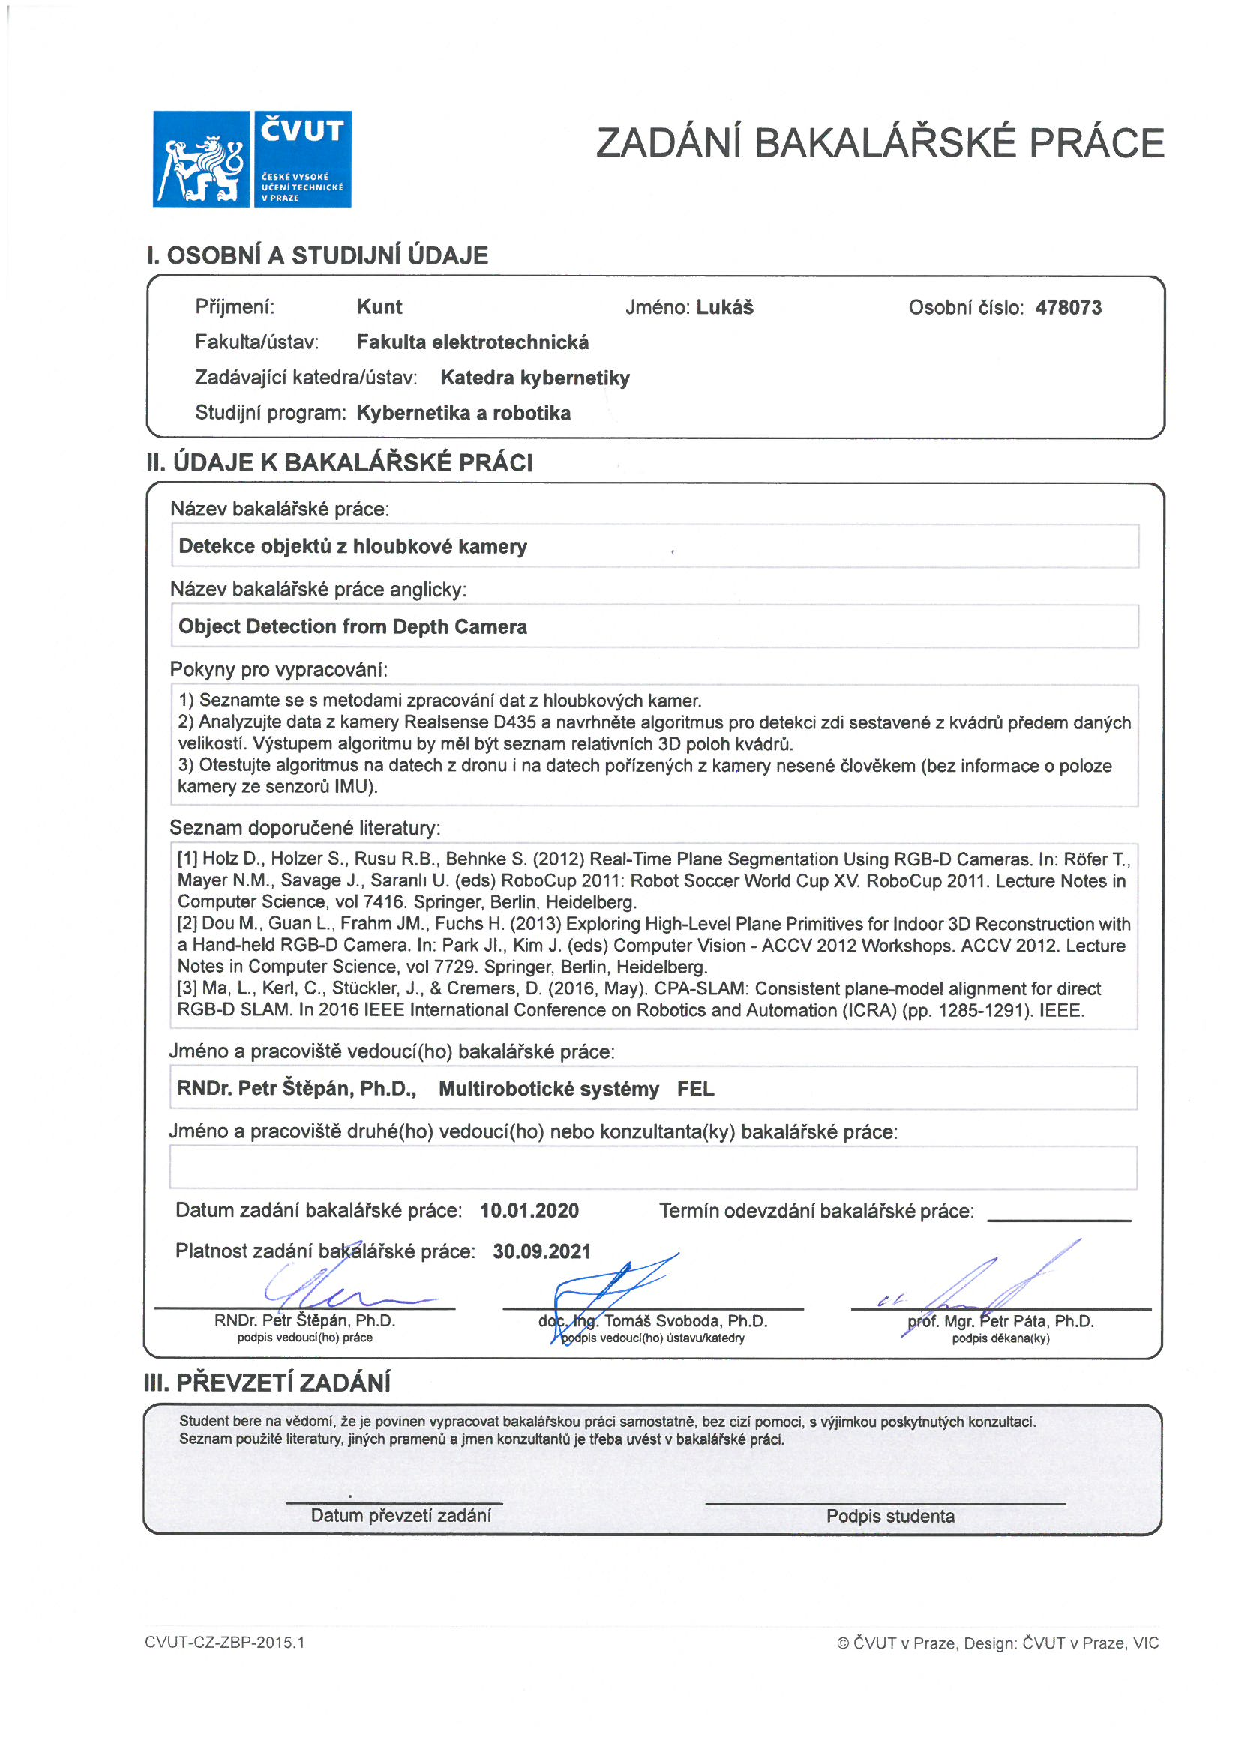
\includepdf{pictures/zadani.pdf}
\section{Homogenní souřadnice}
Během celé práce budeme pracovat jak s kartézskými, tak i s homogenními souřadnicemi. Ty jsou v Euklidovském prostoru dimenze $n$ reprezentovány pomocí vektoru, který má $n+1$ prvků. Je-li $\boldsymbol{r}$ bod v trojdimenzionálním Euklidovském prostoru $\mathbb{E}^3$ reprezentován parametry $x,y,z$, pak pro převod mezi kartézskými a homogenními souřadnicemi platí následující vztahy.
\begin{align}
    \mathbf{r} = \begin{bmatrix} x \\ y \\ z \end{bmatrix} &\rightarrow \mathbf{r}_{hom} = \begin{bmatrix} x \\ y \\ z \\ 1 \end{bmatrix} \\
    \mathbf{r}_{hom} = \begin{bmatrix} x \\ y \\ z \\ w \end{bmatrix} &\rightarrow \mathbf{r} = \begin{bmatrix} \sfrac{x}{w} \\ \sfrac{y}{w} \\ \sfrac{z}{w} \end{bmatrix}
\end{align}
Pomocích homogenních souřadnic můžeme sestavit transformační matici \tl{A}. Ta se skládá z matice rotace \tl{R} a vektoru translace \tl{t}.
\begin{align}
    \mathbf{A} = \begin{bmatrix} \mathbf{R} & \mathbf{t} \\ \mathbf{0} & 1 \end{bmatrix}
\end{align}

\section{Rotace a rotační matice}
Natočení souřadného systému, popřípadě objektu v tomto souřadném systému, vzhledem k jinému souřadnému systému v prostoru dimenze $n$ se nejjednodušeji popíše pomocí rotační matice \tl{R} $\in$ \spc{R}{n}. Mezi nejběžnější rotační matice patří rotace o úhel $\theta$ kolem os kartézského souřadného systému v \spc{E}{3}. Tyto matice vypadají následovně.
\begin{align}
    \mathbf{R_x}=\begin{bmatrix} 1 &  0 & 0 \\ 0 & \cos \theta & -\sin \theta \\ 0 & \sin \theta & \cos \theta \end{bmatrix} \\
    \mathbf{R_y}=\begin{bmatrix} \cos \theta & 0 & \sin \theta \\ 0 & 1 & 0 \\ -\sin \theta & 0 & \cos \theta \end{bmatrix} \\
    \mathbf{R_z}=\begin{bmatrix} \cos \theta & -\sin \theta & 0 \\ \sin \theta & \cos \theta & 0 \\ 0 & 0 & 1 \end{bmatrix}
\end{align}
%\todo{Upravit matice $R_y$ a $R_z$}\\ 
Obecné natočení pak můžeme dostat složením třech a více těchto rotací\footnote{Na pořadí zde záleží. Není možné dostat ,libovolnou rotační matici, pokud budou dvě po sobě doucí rotace probíhat kolem stejné osy.}.
Pro vytvoření matice rotace \tl{R} v prostoru \spc{R}{3} kolem obecné osy dané normalizovaným vektorem \tl{u} o úhel $\theta$ slouží Rodriguesův vzorec \cite{RodriguesRotationFormula}.
\begin{align}
    \mathbf{R} = \mathbf{I} + \tilde{\mathbf{u}}\sin \theta + \tilde{\mathbf{u}}^2(1 - \cos \theta); \quad \tilde{\mathbf{u}} = \begin{bmatrix} 0 & -u_{z} & u_{y} \\ u_z & 0 & -u_x \\ -u_y & u_x & 0 \end{bmatrix}
    \label{Rodriguez}
\end{align}
Chceme-li natočit vektor \tl{a} tak, aby byl rovnoběžný s vektorem \tl{b}, použijeme vzorec \ref{Rodriguez}. Úhel rotace $\theta$ a vektor $\tilde{\mathbf{u}}$, kolem kterého rotace proběhne, se určí následovně.
\begin{align}
    \tilde{\mathbf{u}} = \frac{\mathbf{a} \times \mathbf{b}}{\norm{\mathbf{a}\times \mathbf{b}}} \label{eq:vector_rogrig}\\
    \theta = \arccos \left( \frac{\mathbf{a} \cdot \mathbf{b}}{\norm{\mathbf{a}}\norm{\mathbf{b}}} \right) \label{eq:angle_rogrig}
\end{align}
Podle Walkera \cite{james_w_angle_2014} je tato metoda nevhodná pro výpočet na počítači. Zejména pak v případech, kdy bychom měli počícat $\arccos$ hodnot blízko $\pm 1$. Toto je způsobeno omezenou přesností reprezentace desetinných čísel v počítači (takzvaná floating point aritmetika). Přesnější je tedy použít vzorec
\begin{align}
    \theta = \text{atan2}\left( \norm{\mathbf{a} \times \mathbf{b}}, \mathbf{a}\cdot \mathbf{b} \right).
\end{align}
Výhoda funkce atan2 oproti arcus tangens je ošetřené dělení nulou, ke kterému může dojít při zaokrouhlování desetinných čísel. Navíc výstupem funkce je úhel v rozmezí $\left[ 0, 2\pi \right)$.

\section{Sobelův operátor pro detekci hran}
\label{subsec:sobel}
Hrana v obrazu může být pozorována jako prudká změna intenzity obrazu v daném místě. Rychlé změny se dají detekovat pomocí gradientu, který je pro spojitou funcki $f(x,y)$ v bodě $(x,y)$ vyjádřen následovně. 
\begin{align}
    \nabla f(x,y) =  \begin{bmatrix} \mathbf{G}_x & \mathbf{G}_y \end{bmatrix} = \begin{bmatrix} \frac{\partial f}{\partial x} & \frac{\partial f}{\partial y} \end{bmatrix} \label{eq:grad}
\end{align}
Velikost a směr gradientu se určí pomocí následujících vztahů.
\begin{align}
    \text{mag}(\nabla f) = ||\nabla f ||_2 = \sqrt[2]{\mathbf{G}_x ^2 + \mathbf{G}_y ^2} \label{eq:grad_mag} \\
    \boldsymbol{\theta} = \text{arctan} (\frac{\mathbf{G}_y}{\mathbf{G}_x})
\end{align}
Parciální derivace musí být spočtené pro každý pixel $(x,y)$ obrazu \tl{A}. K tomuto se využívá Sobelových kernelů $\mathbf{K}_x$, $\mathbf{K}_y$. Ty se konvolvují s obrazem a v každém bodě aproximují hodnotu obou parciálních derivací $g_x(x,y), g_y(x,y)$, ze kterých se pak dle vztahu \ref{eq:grad} určí gradient.
\begin{align}
    \mathbf{K}_x = \begin{bmatrix} -1 & 0 & 1 \\ -2 & 0 &2 \\ -1 & 0 & -1 \end{bmatrix} \quad \mathbf{K}_y = \begin{bmatrix} 1 & 2 & 1 \\ 0 & 0 & 0 \\ -1 & -2 & -1 \end{bmatrix} \\
    g_x(x,y) = \sum_{k = -1}^1 \sum_{l = -1}^1 \mathbf{K}_x(k,l)\mathbf{A}(x+k, y+l) \\
    g_y(x,y) = \sum_{k = -1}^1 \sum_{l = -1}^1 \mathbf{K}_y(k,l)\mathbf{A}(x+k, y+l) \\
\end{align}
Určení gradientu intenzity tímto způsobem je relativně nenáročné. Pro zrychlení výpočtu se používá aproximace magnitudy gradientu místo exaktního výpočtu \ref{eq:grad_mag}. Nejjednodušší aproximací je 
\begin{align}
    \text{mag}(\nabla f) \approx ||\nabla f ||_1 = |\mathbf{G}_x| + |\mathbf{G}_y|.  
\end{align}
Ta dává sice velice nepřesný výsledek, ale pro aplikace, kde stačí hrubý odhad velikosti gradientu, může značně snížit výpočetní dobu.\cite{gao2010improved,jin2009edge}

\section{Hledání konvexního obalu množiny bodů}
Je-li dána množina $S$ obsahující $n$ bodů v euklidovském prostoru $\mathbb{E}^3$, popřípadě euklidovské ploše $\mathbb{E}^2$, pak konvexní obal $H$ množiny $S$ je nejmenší konvexní možina obsahující množinu $S$.\cite{chan1996optimal}

Mezi nejpoužívanější algoritmy pro hledání konvexního obalu bodů v  euklidovské ploše $\mathbb{E}^2$ patří následující.
\subsection{Grahamův algoritmus}
Je nalezen bod $\mathbf{p}_0$, jehož $y$-ová souřadnice nabývá nejmenší hodnoty ze všech bodů množiny $S$. Všechny ostatní body jsou seřazeny podle úhlu, který svírají s osou $x$. K tomuto se využívá obecného třídícího algoritmu, jako je například heapsort, a tento krok má tedy časovou náročnost $\mathcal{O}(n\log n)$. Seřazené body jsou postupně procházeny a na základě následujícího kritéria zařazeny\footnote{Bod zařezený do konvexního obalu může být v dalším kroku vyloučen.}, popřípadě vyloučeny, z konvexního obalu $H$ 
        \begin{align}
            \begin{gathered}
            O(\mathbf{p}, \mathbf{r}, \mathbf{q}) = \det \begin{pmatrix} p_x & r_x & q_x \\ p_y & r_y & q_y \\ 1 & 1 & 1 \end{pmatrix}, \\
            \left\{ \begin{gathered}
                    \mathbf{r} \in H, \mathbf{p} = \mathbf{r}, \mathbf{r} = \mathbf{q}, \mathbf{q}  = \mathbf{p_i} \text{ iff } O > 0 \\
                    \mathbf{r} \notin H, \mathbf{p} = \mathbf{p}, \mathbf{r} = \mathbf{q}, \mathbf{q}  = \mathbf{p_i} \text{ iff } O \leq 0
            \end{gathered} \right\},
        \end{gathered}
        \end{align}
kde $\mathbf{p}_i$ je další bod v pořadí seřazených bodů z $S$. Výše popsané ověřování bodů je provedeno v čase $\mathcal{O}(n)$.\cite{convex_hull_formalizing}


Na podobném principu funguje i Andrewův algoritmus. Ten využívá lexikografického uspořádání bodů podle $x$-ové souřadnice, čímž se vyhne výpočtům s destinnou čárkou, které mohou být zdrojem nepřesností.\cite{convex_hull_review}

\subsection{Jarvisův pochod (Jarvis march)}
Je zvolen bod $\mathbf{p}_0$ náležící konvexnímu obalu $H$, což je například první bod v lexikografickém uspořádání bodů $S$. Ten je možné najit v čase $\mathcal{O}(n)$. Dále je spočítán relativní úhel mezi $\mathbf{p}_0$ a ostatními body. Z těch je pak vybrán bod $\mathbf{p}_n$, jehož úhel nabývá nejmenší hodnoty. Bod $\mathbf{p}_n$ je přidán do obalu $H$ a postup se opakuje z bodu $\mathbf{p}_n$. Algoritmus končí ve chvíli, kdy platí $\mathbf{p}_n = \mathbf{p}_0$. Tento postup odpovídá postupnému procházení všech vrcholů polygonu, který reprezentuje konvexní obal, a jeho časová náročnost je $\mathcal{O}(hn)$, kde $h$ je počet vrcholů. Může tedy být pro aplikace s předem známým počtem vrcholů rychlejší než Grahamův algoritmus.

\subsection{Chanův algoritmus}
Jedná se o ideální na výstup citlivý algoritmus určený k výpočtu konvexního obalu množiny. Výpočet dosahuje náročnosti $\mathcal{O}(n\log h)$ 

Množina bodů  $S$ je rozdělena do $K$ množin $Q_i$. V každé množině se nachází maximálně $m$ bodů, kde $m$ je předem určená hodnota, pro kterou musí platit $m \geq h$. Pokud tato rovnost není splněna, musí být hodnota $m$ zvýšena a algoritmus se opakuje. Následně je proveden Grahamův algoritmus na každou množinu $Q_i$ s časovou náročností $\mathcal{O}(n\log m)$. Poté je zvolen bod, který náleží $H$ a je užit Jarvisův pochod. Ten musí najít nejmenší prvek mezi maximálně $m$ seřazenými vrcholy v $K$ množinách, což je realizovatelné v čase $\mathcal{O}(K \log m)$. Pro $h$ vrcholů je tedy výsledná časová náročnost $\mathcal{O}(n \log h)$ za předpokladu, že hodnota $m$ je blízká hodnotě $h$.\cite{chan1996optimal}

\section{Nejmenší ohraničující obdélník}
\label{sec:nejmenší_obdélník}
Nejmenší ohraničující obdélník je možné určit z konvexního obalu $H$ množiny $S$. Ten může být nalezen v čase $\mathcal{O}(h)$ například pomocí star algoritmu \cite{toussaint1984complexity} nebo pomocí algoritmu otáčejících se třmenů (rotating calipers).

Kolem množiny jsou umístěny dva páry na sebe ortogonální přímek, takzvaných třmenů (viz. obrázek \ref{fig:rotating_calipers}), které se konvexního obalu dotýkají v některém z vrcholů $\mathbf{p}_i$, nebo mají společnou přímku spojující vrcholy \tli{p}{i-1} a \tli{p}{i}. V každém kroku je spočítán úhel \tli{\theta}{i} mezi třmenem, který se dotýká vrcholu \tli{p}{i}, a vrcholem \tli{p}{i+1}. Tento výpočet se opakuje pro všechny 4 třmeny, viz. obrázek \ref{fig:rotating_calipers}. Následně je výbrán úhel $\theta = \min \{ \theta_i, \theta_j, \theta_k, \theta_l \}$, o který je provedena rotace všech třmenů. Třmeny jsou pak ve směru svého normálového vektoru posunty tak, aby platila výše uvedená podmínka dotyku třmenu s konvexní množinou v jednom, resp. dvou vrcholech. Dále je vypočten obsah obdélníku, jehož strany tvoří výše zmíněné třmeny. Celý postup se poté opakuje, dokud není vyzkoušeno všech $h$ obdélníků. Následně je vybrán ten s nejmenší plochou. \cite{toussaint1984complexity}

\begin{figure}
    \centering
    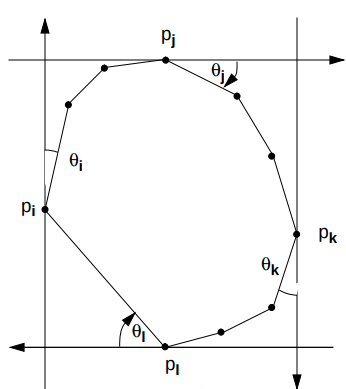
\includegraphics[width = 0.5\linewidth]{pictures/rotating_calipers.png}
    \caption{Otáčející se třmeny \cite{toussaint1984complexity}}
    \label{fig:rotating_calipers}
\end{figure}

\section{Matematická morfologie ve zpracování obrazu}
\label{sec:morphology}

Matematická morfologie zpracovává obraz v závislosti na jeho tvaru. Jejím účelem je zjednodušit obraz při zachování základního tvaru a potlačení nepodstatných informací obsažených v obrazu \cite{haralick1987image}. K filtraci obrazu se využívá strukturní element $H$. Tento element slouží jako lokální sonda, citlivá na geometrickou informaci. Příklad strukturních elementů je na obrázku \ref{fig:sondy}, kde symbolem $\times$ je znázorněn lokální počátek, ke kterému je element $H$ vztažen. Základními morfologickými operacemi jsou: dilatace, eroze, otevření a uzavření. Tyto operace jsou reprezentovány symboly $\oplus, \ominus, \circ, \bullet$.


Morfologické operace mohou být definovány pro binární, černobílý i barevný obraz. Nechť $X \subseteq \mathbb{Z}^2$ je binární obraz, pak základní morfologické operace jsou definovány následovně.\cite{comer1999morphological}
\begin{align}
    X \oplus H = \{ (x,y): H_{(x,y)} \cap X \neq \emptyset \} \\
    X \ominus H = \{ (x,y): H_{(x,y)} \cap X \subseteq X \} \\
    X \circ H = (X \ominus H) \oplus H \\
    X \bullet H = (X \oplus H) \ominus H
\end{align}
Kde jako $H_{(x,y)}$ je označena sonda $H$, jejiž počátek byl posunut do bodu $(x,y)$.

\begin{figure}
    \centering
    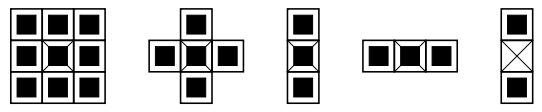
\includegraphics[width = \linewidth]{pictures/sondy_morfologie.png}
    \caption{Běžné sondy používané při v matematické morfologii}
    \label{fig:sondy}
\end{figure}
%\todo[inline]{Popsání základních morfologických operací jako je dilatece, eroze, ...}

\section{Random sample consensus}
\label{sec:ransac}
Při určování modelu podle statistických metod, jako je prokládaní pomocí nejmenších čtverců, může jediný bod zatížený velkou chybou znehodnodit aproximaci matematickým modelem. Příklad takové situace je vidět na obrázku \ref{fig:least_squares_error}.
Iterativní algoritmus Random sample consensus (RANSAC) je vhodný v situacích, kde jsou data zatížena velkým množstvým chybových bodů, popřípadě body s velkou magnitudou chyby. Princip algoritmu je následující: \cite{derpanis2010overview}

\begin{algorithm}
    \caption{RANSAC}
    \label{alg:RANSAC}
    \begin{algorithmic}[1]
        \STATE Je náhodně vybrán minimální počet bodů potřebných k určení parametrů modelu.
        \STATE Jsou nalezeny parametry modelu.
        \STATE Je určeno kolik bodů z množiny $S$ je od modelu vzdáleno maximálně $\epsilon$. 
        \STATE Pokud poměr bodů určených v kroku 3 ku celkovému počtu je větší než předem určený limit $\tau$, pak algoritmus končí a model je určen z bodů určených v bodě 3.
        \STATE Jinak jsou kroky 1 až 4 jsou opakovány až $n$ krát.
        \STATE Pokud během $n$ běhů nebyl algoritmus ukončen, je vybrán model, pro který byl počet bodů získených v kroku 3 největší.
    \end{algorithmic}
\end{algorithm}

\begin{figure}
    \centering
    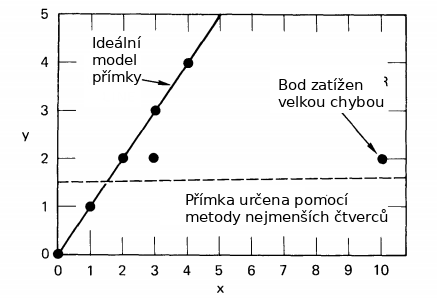
\includegraphics[width = 0.6 \linewidth]{pictures/ransac_least_squares.png}
    \caption{Vliv bodu zatíženého chybou na prokládaní přímky pomocí nejmenších čtverců \cite{fischler1981random}}
    \label{fig:least_squares_error}
\end{figure}
Algoritmus tedy není deterministický a je citlivý na správné nastavení jednotlivých parametrů. Zejména pak na počet opakování $n$. Tento se parametr se volí experimentálně. Pokud je známa provděpodobnost výskytu chybového bodu, pak můžeme parametr $n$ určit na základě požadované pravděpodobnosti $p$, že alespoň jedna sada náhodných vzorků neobsahuje bod zatížený velkou chybou (tzv. outlier). Pokud jako $v$ označíme pravděpodobnost bodu s velkou chybou a $u$ bod jehož chyba není markantní, pak platí následující vztahy. \cite{fischler1981random}
\begin{align}
    1 - p = (1 - u^m)^N \\
    n = \frac{\log(1 - p)}{\log(1 - (1 - v)^m)}
\end{align}
Písmenem $m$ je označen počet bodů potřebný k určení modelu. 


%\todo[inline]{popsání funkce ransac algoritmu}

%\section{Vlastní čísla a vektory}
%Pro čtvercovou matici \minsp{A}{R}{n\times n} a nenulový vektor \tl{v}\minsp{}{R}{n} a sklár $\lambda \in \mathbb{R}$ platí
%\begin{align}
    %\mathbf{Av} = \lambda \mathbf{v}.
%\end{align}
%Skalár $\lambda$ se nazývá vlastní číslo matice \tl{A} a vektor \tl{v} vlastní vektor příslušný vlastnímu číslu $\lambda$.
%Spektrální věta (viz. \cite{Werner2020}) říka: Je-li matice \tl{A} symetrická, pak má $n$ vlastních čísel, kde $n = \text{rank}\mathbf{A}$ a všechna vlastní čísla jsou reálná.
%\todo[inline]{Bude upraveno podle toho, co bude potřeba na popsání funkce PCA, SVD a ortogonální projekce}


%\section{Singulární rozklad}
%\todo[inline]{Stručně posat singulární rozklad PCA a ortogonální projekci na podprostor}
%Singulární SVD\footnote{Z anglického Singular Value Decomposition}rozklad umožní každou matici \tl{A} $\in$ \spc{R}{m \times n} rozložit jako
%\begin{align}
    %\mathbf{A} = \mathbf{USV}^T
%\end{align}
%kde matice \tl{S} je diagonální, matice \tl{U} je ortogonální a obsahje vlastní vektory matice \tl{AA}$^T$, obdobně je pak i matice \tl{V} ortogonální a je složena z vlastních vektorů matice \tl{A}$^T$\tl{A}

%\section{Ortogonální projekce na podprostor}
%\label{sec:projekce}

%\section{Analýza hlavních komponent}
%%Analýza hlavních komponent (PCA\footnote{Z anglického Principal Component Analysis}) 


\chapter{Kamera}

\section{Dírkový model kamery}
Kamera zobrazuje body euklidovského prostoru $\mathbb{E}^3$, které jsou popsány pomocí světových souřadnic, na body v euklidovské ploše $\mathbb{E}^2$, která se nazývá obraz. Body obrazu se označují jako pixely. 

Nejjednodušším modelem kamery je model dírkový, který má optické centrum, neboli centrum projekce, v konkrétním bodě. Centrum projekce umístíme do počátku kartézského souřadného systému a budeme uvažovat plochu kolmou na osu $Z$ našeho souřadného systému, kterou nazveme obrazovou rovinou. Ta je popsána jediným parametrem a to ohniskovou vzdáleností $f$. V dírkovém modelu kamery se bod \tl{p} = $(x,y,z)^T$ v prostoru promítne na bod obrazu pomocí zobrazení
\begin{align}
    \begin{bmatrix} x \\ y \\ z \end{bmatrix} \mapsto \begin{bmatrix} \sfrac{fx}{z} \\ \sfrac{fx}{z} \end{bmatrix},
    \label{pinhole_eq}
\end{align}
což odpovídá bodu, kde přímka spojující centrum projekce a bod v prostoru protne obrazovou rovinu (viz obrázek \ref{pinhole}). Ve vztahu \ref{pinhole_eq} jsme předpokládali, že počátek souřadného systému obrazu je v optickém středu. Konvencí však je za počátek souřadnic zvolit levý horní roh obrazu. K zápisu využijeme homogenních souřadnic a dostaneme následující rovnici 
\begin{align}
    \begin{bmatrix} x \\ y \\ z \\ 1 \end{bmatrix} \mapsto \begin{bmatrix} fx + zc_x \\ fy + zc_y \\ z \end{bmatrix} = \begin{bmatrix} f & 0 & c_x & 0 \\ 0 & f & c_y & 0 \\ 0 & 0 & 1 &0 \end{bmatrix} \begin{bmatrix} x \\ y \\ z \\ 1 \end{bmatrix},
    \label{eq:pinhole_homogenous}
\end{align}
kde jsme jako $c_x$ a $c_y$ označili souřadnice optického středu. Označíme-li obecný bod v prostoru, který je popsán v souřadném systému kamery, \tl{x}$_p$ a odpovídající bod v rovině obrazu \tl{x}, pak můžeme rovnici \ref{eq:pinhole_homogenous} přepsat jako
\begin{align}
    \mathbf{x} = \mathbf{K}[\mathbf{I}\; |\; 0 ]\mathbf{x}_p \quad \mathbf{K} = \begin{bmatrix} f & 0 & c_x  \\ 0 & f & c_y  \\ 0 & 0 & 1  \end{bmatrix}.
    \label{intrinstic}
\end{align}
Matice \tl{K} se nazýva matice vnitřních parametrů kamery.

Obecně je bod $\mathbf{x}$ v euklidovském prostoru popsán v jiném souřadném systému, než je ten se kterým je svázána kamera. Tento souřadný systém se nejčastěji nazývá světový. Přechod do souřadného systému kamery ze světového je možno popsat následovně 
\begin{align} 
    \mathbf{x}_p = \begin{bmatrix} \mathbf{R} & -\mathbf{R\tilde C} \\ 0 & 1 \end{bmatrix}
    \mathbf{x}.
    \label{eq:world_to_cam}
\end{align}
Jako $\tilde{\mathbf{C}}$ jsme označili počátek souřadného systému kamery vyjádřený v světových souřadnicích a \tl{R} rotaci světového souřadného systému vzhledem ke kameře. Dosadíme-li nyní rovnici \ref{intrinstic} do \ref{eq:world_to_cam} dostaneme vztah popisující transformaci bodu ze světových souřadnic do souřadnic obrazu
\begin{align}
    \mathbf{x} = \mathbf{KR}[\mathbf{I} \; | \; - \mathbf{\tilde C} ]\mathbf{x}.
    \label{eq:world_to_img}
\end{align}
Parametry $\mathbf{\tilde C}$ a \tl{R} se souhrně nazývají vnější parametry kamery. 
\begin{figure}
    \centering
    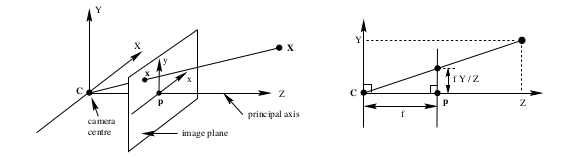
\includegraphics[width = 0.8\linewidth]{pictures/dirkovymodel_nakres.png}
    \caption{Model dírkové kamery}
    \label{pinhole}
\end{figure}

\section{Stereo kamera}
\subsection{Výpočet vzdálenosti}
Stereo kamera je tvořena dvěmi nezávislými čočkami. Zpracováním obrazů z obou čoček jsme schopni získat informace o hloubce každého pixelu\footnote{Hloubkou bodu \tl{p} je myšlena vzdálenost ortogonální projekce \tl{p} na optickou osu kamery od počátku souřadného systému, který je svázan s kamerou.}. Budeme uvažovat model stereokamery, kde jsou osy obou čoček rovnoběžné (viz obrázek \ref{stereo_paralel}). Osy jsou od sebe ve vzdálenosti $b$. Tomuto parametru se říka báze (baseline). Z podobnosti trojúhelníků plyne
\begin{align}
    \frac{z}{f} = \frac{x}{xl} \label{trojuh1} \\
    \frac{z}{f} = \frac{x - b}{xr} \label{trojuh2}.
\end{align}
Pokud z rovnice \ref{trojuh1} vyjádříme $x$ a dosadíme do rovnice \ref{trojuh2}, pak po úpravě dostaneme výsledný vztah pro vzdálenost bodu od kamery 
\begin{align}
    z = \frac{fb}{xl - xr} = \frac{fb}{d}.
    \label{depth_stero}
\end{align}
Hodnota $d$ se nazývá rozdíl (disparity) a $xl$, $xr$ jsou souřadnice bodu \tl{p} v levém, resp. pravém obrazu stereokamery. Pro každý bod v levém obrazu je tedy potřeba najít odpovídající bod v obrazu pravém (tzv. stereo pár). Bez jakékoliv apriorní znalosti by to znamenalo pro každý pixel prohledat celý druhý obraz, tedy náročnost hledání $\mathcal{O}(n^2)$, kde $n$ odpovídá velikosti strany obrazu v pixelech. Pomocí epipolární geometrie můžeme hledání zúžit na přímku  a snížit tak náročnost hledání stereo páru na $\mathcal{O}(n)$. \cite{brown2003advances_in_stereo}

\subsection{Chyba výpočtu vzdálenosti}
Chyba výpočtu vzdálenosti se určí derivací rovnice \ref{depth_stero} podle $d$ \cite{keselman2017intel} 
\begin{align}
    \frac{\partial z}{\partial d} = \frac{z}{fb} \\
    |\epsilon_z | = \frac{z^2}{fb}|\epsilon_d |,
    \label{error_stereo}
\end{align}
kde $\epsilon_z $ je chyba určení vzdálenosti bodu a $ \epsilon_d $ je chyba rozdílu. Tato chyba je vlastností kamery, popřípadě algoritmu použitého ke hledání odpovídajících párů, a nabývá téměř konstantních hodnot \cite{keselman2017intel}. Z rovnice \ref{error_stereo} tedy plyne, že chyba je úměrná kvadrátu vzdálenosti daného bodu a přesnost stereokamer se vzdáleností rychle klesá.

\subsection{Epipolární geometrie}
\label{Sec:epipolar}
Epipolární geometrie se zabývá průnikem obrazových rovin se svazkem ploch, jejichž společná osa je báze. Uvažujme dvě dírkové kamery v obecném natočení, tedy jejich obrazové roviny nemusí být rovnoběžné, viz \ref{fig:epipolar}. Z dírkového modelu kamery plyne, že bod \tl{X}, který se nachází v euklidovském prostoru, a optické středy kamer $C, C'$ jsou koplanární a tvoří rovinu $p$. V místě, kde tato rovina protíná roviny obrazu, se nachází epipolární přímky \tl{l} a $\mathbf{l'}$\footnote{Přímky tl{l} a \tl{l'} jsou popsány pomocí homogenních souřadnic.}. Hledáme-li stereo pár, pak pro známý bod \tl{x} (tj. projekce bodu \tl{X} do optické roviny levé kamery) musíme najít odpovídající bod \tl{x'}. Ten může ležet pouze na epipolární přímce \tl{l'}, která je jednoznačně určena epipólem \tl{e'} a bodem \tl{x'}. Epipól se nachází v místě, kde přímka spojující optická centra kamer, protíná rovinu pravého obrazu. Pro bod \tl{x'} platí
\begin{align}
    \mathbf{x'} = \mathbf{Hx},
\end{align}
kde \tl{H} je homografie mezi rovinami obrazu. Toto zobrazení je ovlivněno pouze vzájemnou polohou kamer a jejich vnitřními parametry. Nezávisí tedy na scéně.
Z bodu \tl{x'} lze určit epipolární přímku 
\begin{align}
    \mathbf{l'} = \mathbf{e'} \times \mathbf{x'} \\
    \mathbf{l'} = \mathbf{e'} \times \mathbf{Hx} \\
    \mathbf{l'} = \mathbf{Fx}.
\end{align}    
Matice \tl{F} se nazývá fundamentální a představuje zobrazení $f:\mathbb{R}^3 \mapsto \mathbb{R}^3$.
Pokud jsou obě optické osy stereokamery rovnoběžné, pak se výpočet epipolární přímky velice zjednoduší, jelikož homografie mezi rovinami obrazu je pouze posunem ve směru báze. \cite{hartley2004multiple}
\begin{figure}
    \centering
    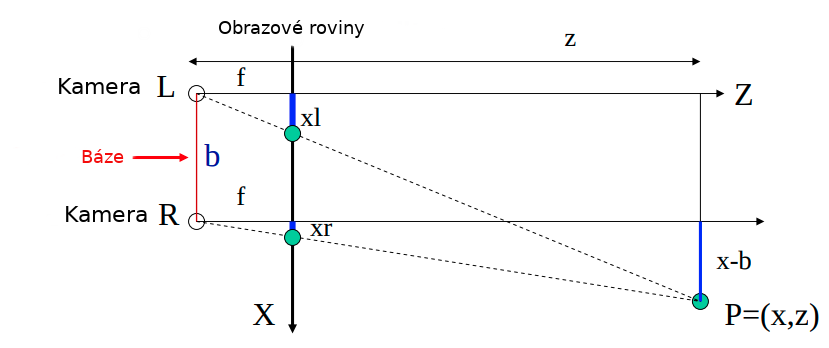
\includegraphics[width = 0.8\linewidth]{pictures/stereo_sketch.png}
    \caption{Určení vzdálenosti bodu ze stereokamery, převzato z \cite{washingtion_steropic}}
    \label{stereo_paralel}
\end{figure}
\section{Hledání stereo páru}
Metody užívané pro hledání stereo páru se dělí na metody plošné (area based) a metody založené na porovnávání rysů (features). Při hledání stereo páru se často využívá následujících omezení, která tento proces zjednoduší. Tato omezení však v extrémních případech, jako je například okluze,  nemusí platit.
\begin{itemize}
    \item Epipolární omezení: Pixel v druhém obrazu se nachází ( pokud existuje ) na epipolární přímce, viz. sekce \ref{Sec:epipolar}.
    \item Spojitost: Rozdílová, popř. hloubková, mapa by měla být po částech spojitá.
    \item Jedinečnost: Každý pixel v levém obrazu má k sobě právě jeden odpovídající v obrazu pravém. 
    \item Pořadí: Pořadí pixelů v levém obrazu odpovídá pořadí v pravém.
\end{itemize}
\begin{figure}
    \centering
    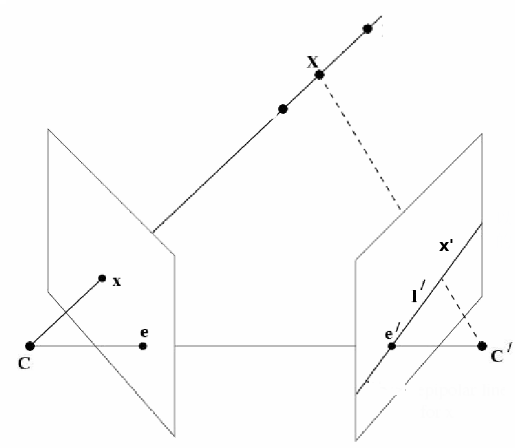
\includegraphics[width = 0.6\linewidth]{pictures/epipolar_g_sketch.png}
    \caption{Projekce bodu na obrazové roviny, převzato z \cite{epipolar_pic}}
    \label{fig:epipolar}
\end{figure}

\subsection{Plošné metody}
Plošné metody využívají informaci z okolí pixelu. Tyto informace jsou porovnány se všemi přípustnými pozicemi v druhém obrazu a bod, jehož hodnota je nejblíže vzoru, tvoří stereo pár. Mezi nejpoužívanější variace plošných metod patří následující.

\subsubsection{Součet absolutních rozdílů}
Je definována konstatní velikost okolí pixelu $\mathbf{x}(u,v)$. Následně jsou hodnoty všech pixelů v okně sečteny a výsledná hodnota je provnána s body v pravém obrazu, kde se může korespondující pixel nacházet, tj. body které splnují námi používaná omezení. Pro odpovídající bod \tl{x'} tedy platí
\begin{align}
    \mathbf{x'} = \text{argmin}\left( \displaystyle\sum_i \displaystyle\sum_j |\mathbf{I}_l(u+i,v+j) - \mathbf{I}_r(u+i, v+j + d)| \right),
\end{align}
kde $\mathbf{I}(u,v)$ je intenzita příslušného pixelu, $d$ je posun okna ve druhém obrazu a součet probíha přes celé okno. Vztah byl zjednodušen uvažováním horizontálních epipolárních přímek. Toto odpovídá konfiguraci kamery s rovnoběžnými optickými osami.

    Existuje mnoho podobných algoritmů, které se liší pouze metrickou funkcí. Místo absolutní hodnoty rozdílu je užit například kvadrát rozdílu  nebo jeho normalizovaný kvadrát. Jedná se o nejrychlejší algoritmy pro hledání stereo páru, přesto však dosahují vysokých přesností. \cite{kuhl2005comparison, hartley2004multiple} 

\subsubsection{Cenzus}
\label{Sec:cenzus}
Jedná se o algoritmus patřící do rodiny plošných metod, které před porovnáním hodnot pixelů provedou určitou transformaci obou obrazů. Patří sem naříklad i transformace podle hodnoty (rank transform). Cenzus opět pracuje s definovanou maskou kolem pixelu, pro který hledá stero pár. Pixely, které se nachází v šabloně, se transformují na vektor jedniček a nul podle toho, zda je hodnota intenzity pixelů masky větší, popřípadě menší, než intenzita centrálního pixelu. Stejná transformace se provede i v pravém obrazu pro každý pixel, který může doplnit stereo pár. Vektory jsou následně porovnány a je vybrán ten, jehož vektor má nejmenší Hammingovu vzdálenost \cite{kuhl2005comparison, brown2003advances_in_stereo}.

\subsection{Porovnávání rysů}
Pro každý obraz jsou vygenerovány důležité body. To mohou být například hrany či rohy v obrazu. Tyto rysy jsou porovnány s analogicky vygenerovánými rysy v druhém obrazu. Tento postup se v některých aplikacích opakuje, přičemž v každém dalším kroku je každý rys rozložen na několik menších, o kterých již máme apriorní znalost jejich přibližné polohy. Aby bylo možné sestavit obraz pouze z několika rysů, je nutné provést časově náročné předzpracování obrazu za účelem najití vhodných rysů a po nalezení korespondujících rysů provést zpětnou rekonstrukci obrazu. \cite{brown2003advances_in_stereo}

%\todo[inline]{dolnit }
Pro porovnání rysů mezi levým a pravým obrazem se využívá algoritmů jako je například SIFT , SURF  nebo BRIEF.

%TODO uncoment this ( avoiding compilation warnings )




%\section{Intel \textregistered Realsense\textsuperscript{TM} D435}
\section{Intel Realsense D435}
Intel\textregistered{} Realsense\textsuperscript{TM} D435 je širokoúhlá stereokamera, která se skládá z RGB kamery, infračerveného projektoru a dvou infračervených kamer, jejichž data jsou zpracovává přímo v čipu kamery dedikovaným procesorem. Výstupem z kamery je tedy barevný obraz a vzdálenost jednotlivých pixelů, neboli hloubková mapa. 

\begin{figure}
    \centering
    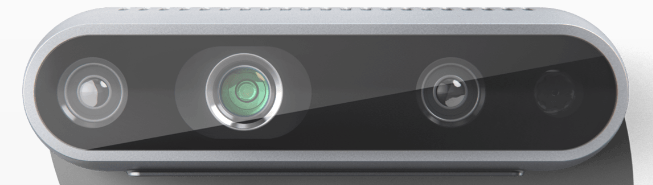
\includegraphics[width = 0.8\linewidth]{pictures/realsense_kamera.png}
    \caption{Fotografie kamery Intel\textregistered{} Realsense\textsuperscript{TM} D435 \cite{Realsense_obrazek}}
    \label{Fig:realsense_pic}
\end{figure}

Dvě infračervené kamery jsou v konfiguraci s rovnoběžnými optickými osami ve vzdálenosti 50$\,\si{mm}$. Infračervený projektor promítá na scénu statický obrazec, který se nachází mimo viditelné spektrum a není tedy zachycen RGB kamerou. Tento obrazec slouží k nalezení stereo párů, zejména u objektů s řídkou texturou.

    Kamera je vybavena specializovaným procsorem Vision Processor D4 pro výpočet hloubkové mapy. Ten je schopen při rozlišení hloubkové kamery 848x480 zpracovávat až 90 snímků za sekundu. Při této rychlosti snímání je přesnost kamery výrazně snížena \cite{keselman2017intel}. Pro maximální přesnost je vhodné nastavit frekvenci na 30 snímků za sekundu. 
    
    Procesor má stejně jako celá kamera velice nízký odběr elektrické energie. Celá kamera včetně IR projektoru má odběr menší než jeden watt a je tedy vhodná pro mobilní aplikace, kde je velikost baterie a spotřeba energie omezujícím faktorem \cite{RealSense_datasheet}. %\todo[inline]{Porovnání s Kinectem a Asus RGBD kamerou}

    Pro hledání stereo párů je využit algoritmus Cenzu popsaný v \ref{Sec:cenzus} s maskou o velikosti $7 \times 7 $. Výsledky jsou následně ověřovány sadou filtrů, které měří důvěryhodnost shody. Podle nastaveného limitu důvěryhodnosti pak pro tento pixel buď vygenerují záznam v hloubkové mapě, nebo pixel zůstane nevyplněn. Výsledky kamery pro různé hodnoty limitu jsou vidět v tabulce \ref{tab:tablka_limity}. 
\begin{table}[h]
    \centering
    \begin{tabular}{|c|c|c|c|} \hline
        Důvěryhodnost & FPR & $r_p = 95\%$ & max($\sigma_x,\sigma_y$)\,>\,$\sigma_z$ \\ \hline \hline
        Vypnuta & 91,3\% & 7.0\,m & 6.1\,m \\ \hline
        Nízká & 19,8\% & 6,9\,m & 6.6\,m \\ \hline
        Střední & 5,8\% & 5,8\,m & 6.7\,m \\ \hline
        Vysoká & 0,5\% & 4,2\,m & 6.8\,m \\ \hline
    \end{tabular}
    \caption[Výstup kamery v závislosti na nastavené důvěryhodnosti]{Výstup kamery v závislosti na nastavené důvěryhodnosti. Postupně zleva: Hodnota limitu, počet falešných shod pokud je scéna blíže než je minimální vzdálenost detekce kamerou. Vzdálenost, kdy vyplněnost hloubkové mapy klesne pod $95\%$, a vzdálenost při které je směrodatná odchylka ve směru osy $z$ menší než ve směru $x$ a $y$. Převzato z \cite{keselman2017intel}.}
    \label{tab:tablka_limity}
\end{table}
%\begin{figure}
    %\centering
    %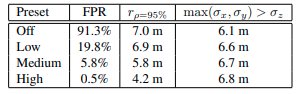
\includegraphics[width = 0.8\linewidth]{pictures/realsense_threshold.png}
%\end{figure}

Procesor kamery není schopen určit hloubku bodů, pokud se objekt nachází příliš blízko. Konkrétní hodnoty je možno vidět v tabulce \ref{tab:minimalni_hloubka}. Maximální měřitelná vzdálenost je za ideálních podmínek až 40 metrů \cite{keselman2017intel}. S rostoucí vzdáleností se kamera chová podle rovnice \ref{error_stereo} a přesnost tedy rychle klesá. Toto chování neodpovídá rovnici \ref{error_stereo}, pokud kamera operuje s objekty, které se nachází na obou hranicích měřitelné vzdálenosti. Ilustrace výstupu kamery, pokud se objekt nachází ve vzdálenosti meší než specifikuje tabulka \ref{tab:minimalni_hloubka}, je vidět na obrázku \ref{fig:rs_bad}.

%\begin{figure}
    %\centerin,g
    %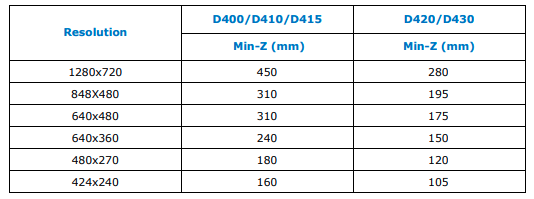
\includegraphics[width = 0.8\linewidth]{pictures/minimalni_vzdalenost.png}
%\end{figure}

\begin{table}
    \centering
    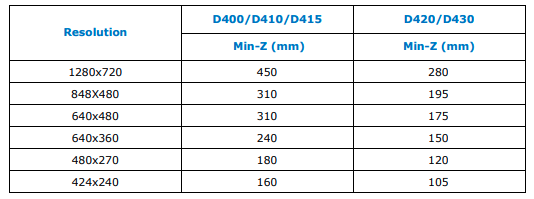
\includegraphics[width = 0.8\linewidth]{pictures/minimalni_vzdalenost.png}
%\end{figure}
    \caption{Tabulka minimální detekovatelné hloubky \cite{RealSense_datasheet}}
    \label{tab:minimalni_hloubka}
\end{table}


\begin{figure}[h]
\centering
\begin{subfigure}{0.48\textwidth}
  \centering
  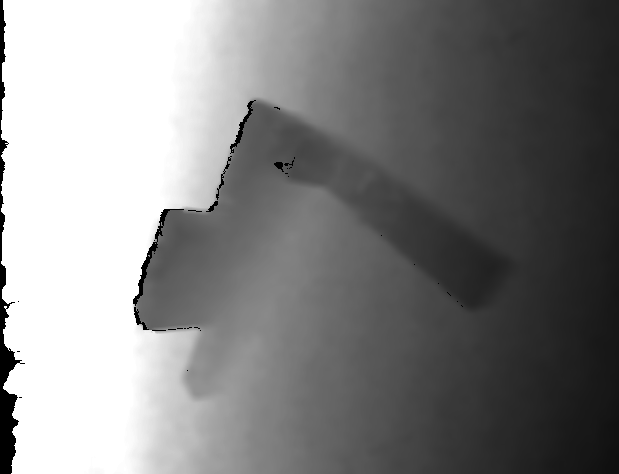
\includegraphics[width=0.9\linewidth]{pictures/good_realsense.png}
  \caption{Snímek bez výrazných výpadků dat hloubkové mapy}
  \label{fig:rs_good}
\end{subfigure}
\begin{subfigure}{0.49\textwidth}
  \centering
  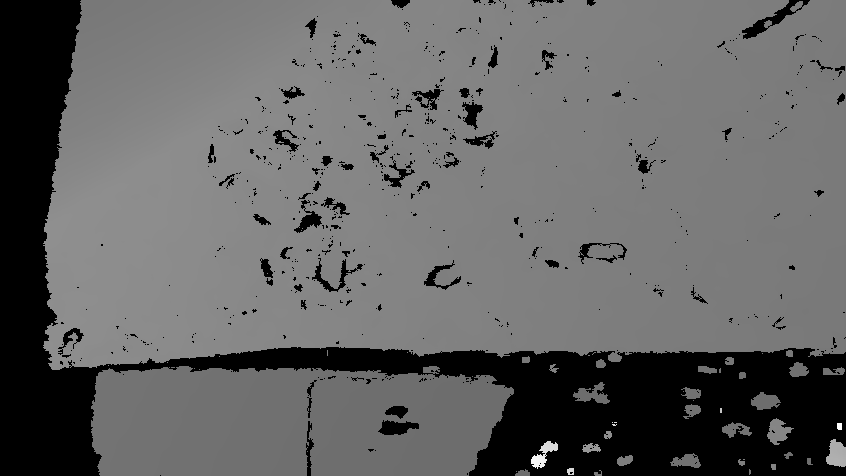
\includegraphics[width=0.9\linewidth]{pictures/bad_realsense.png}
  \caption{Snímek s chybějícími hloubkovými daty}
  \label{fig:rs_bad}
\end{subfigure}
\caption[Výstupní data kamery RealSense]{Výstupní data kamery RealSense, hloubková data byla převedena do odstínů šedé}
\label{fig:realsense_pics}
\end{figure}

\chapter{Metody v detekci objektů z hloubkových dat}
\label{sec:Metody_detekce}
Existuje mnoho různých metod pro detekci objektů z hloubkových dat. Tyto přístupy se liší podle různorodosti detekovaných objektů, požadavků na čas výpočtu, možnosti získání trénovacích dat nebo formátem vstupních dat. Obvyklým formátem je tak zvané mračno bodů (anglicky point cloud), což je nestrukturovaná množina bodů v trojrozměrném prostoru. Zejména v posledních letech s nástupem hloubkových kamer jako je například Microsoft Kinect, Asus Xtion nebo námi používaný Intel RealSense, se čím dál více používájí data ve formátu RGB-D obrazu. Ten se dá pomocí vztahu \ref{eq:pinhole_homogenous} převést na mračno bodů. Výstupní data z hloubkové kamery bývají většinou oproti LIDARu méně přesná. Výhodou naopak je vysoká vzorkovací frekvence, velké množství výstupních bodů a nízká cena zařízení.

\section{Určení normálového vektoru plochy z nestrukturovaných dat}
\label{sec:normal_methods}
Téměř všehny metody detekce objektů z mračna bodů se skládájí z více kroků a jedním ze základních kroků většinou bývá určení normálového vektoru snímané plochy. Obvykle se jedná o plochu reprezentující zem, popřípadě jinou podložku, nebo plochy reprezentující stěny místnosti. Přístupy k hledání ploch v obrazu se výrazně liší, v této práci uvedeme pouze příklady některých z nich.

\subsection{Použití hrubé síly}
Postupně jsou vyzkoušeny všechny možnosti, popřípadě část z nich, a vybere se nejlépe vyhovující. Využívá se zde zejména algoritmů jako je RANSAC, případně jeho modifikace. Tato metoda je vhodná zejména pokud jsou data zatížena silným šumem, jelikož při správném počtu iterací téměř vždy vrátí správný výsledek. Toto je však vykoupeno vysokou časovou náročností \cite{RANSAC_plane,single_RGBD_reconstruction}, která se dá snížit vhodným předzpracováním dat, například segmentací na menší celky a určením plochy pouze pro tyto segmenty. \cite{rusu2009close}
\subsection{Výpočet normálového vektoru v každém bodě}
Normálový vektor je kolmý na plochu reprezentující okolí bodu. Toto okolí je tvořeno body nacházejícími se v okruhu o poloměru $r$ \cite{wang2015dominant} ,popřípadě $k$ nejbližšími body\cite{holz2011real,trevor2013efficient}. Poté je provedena segmentace pomocí metody rostoucích oblastí viz. sekce \ref{subsection:segmentation}. Výstupem jsou tedy skupiny bodů, které představují jednotlivé plochy. V některých případech je navíc použit algoritmus RANSAC na již nalezené segmenty za účelem vyloučení bodů, které leží mimo plochu představovanou daným segmentem, přestože jejich normálový vektor dané ploše odpovídá \cite{lai2011large}.
\subsection{Principal Component Analysis}
Jsou nalezeny body, které patří do dané roviny, a těmi je poté pomocí Principal Component Analysis (PCA)\cite{Werner2020} proložena rovina. Tato metoda vyžaduje přesné určení bodů, o kterých se předpokládá, že tvoří danou rovinu. Jediný bod ležící ve velké vzdálenosti od roviny (outlier) může způsobit velké nepřesnosti, jelikož rovina je proložena body metodou nejměnších čtverců, viz obrázek \ref{fig:least_squares_error}.\cite{zhang2016fast}


\section{Segmentace obrazu}
\label{subsection:segmentation}
Důležitým krokem pro porozumění obrazu a detekci objektů je segmentace obrazu, tj. rozdělení vstupních dat na skupiny. Rozdělujeme dva typy segmentace. Sémantickou, která sjednocuje body reprezentující danou skupinu objektů (např. všechny bloky ležící na zemi), a segmentaci jednotlivých instancí, kdy je skupina objektů rozdělena na jednotlivé zástupce dané skupiny. 

    Přístup k segmentaci se líší podle dané aplikce. Nejpoužívanějšími metodami jsou tyto.
    \subsection{Metoda prahování} Body $\mathbf{p}(x,y)$ jsou rozděleny do $m$ skupin podle toho, zda jejich vlastnost $V$, což je například vzdálenost bodu od kamery nebo od plochy, dosahuje stanovené hodnoty $T_m$. Tato hodnota může být pevně určená, nebo se může dynamicky měnit, a to v závislosti na okolních bodech, nebo v závislosti na pozici v obrazu, tj. $T(x,y)$. Pro prahovací metodu tedy platí následující vztah\cite{segmentace_metody}
        \begin{align}
\left\{ 
        \begin{gathered}
            \mathbf{p} \in m \text{ iff } V(\mathbf{p}) > T_m \\
            \mathbf{p} \in n \text{ iff } V(\mathbf{p}) > T_n \\
            \mathbf{p} \in \emptyset \text{ iff } V(\mathbf{p}) \leq T_1 
        \end{gathered}
\right\}.
        \end{align}
 
\subsection{Metoda detekce hran}
V obrazu jsou detekovány prudké změny pozorované vlastnosti $V$ v bodě \tl{p} za pomoci první derivace vlastnosti $V$ v bodě \tl{p}. Pokud hodnota derivace dosáhne daného prahu je \tl{p} registrován jako hrana. Po výpočtu bývá provedena úprava těchto hran, kterou je například filtrování, popřípadě spojení některých sousedních bodů. Nakonec jsou v obrazu identifikovány segmenty bodů, které jsou od zbytku odděleny hranou. K určení hran se využívá například Sobelova operátoru, který byl popsán v sekci \ref{subsec:sobel}, nebo Cannyho operátoru.\cite{single_RGBD_reconstruction}

\subsection{ Metoda rostoucí oblasti}
Metoda rostoucí oblasti se dělí na dva typy. S počátečním bodem (seed) a bez počátečního bodu. 

        Je zvolen jeden, popřípadě několik počátečního bodů. K vybraným bodům se postupně přidávají sousední body, pokud splňují předem definované podmínky. Těmi jsou například maximální odchylka normálových vektorů bodů od normálového vektoru počátečního bodu, nebo rozdíl velikosti některé souřadnice. Metoda bez počátečního bodu pak rozdělí všechny body do skupin, jejichž body spolu sousedí a zároveň mají podobné vlastnoti. Jedná se o algoritmus, který pracuje s konstatní časovou náročností odpovídající $\mathcal{O} (2n)$, kde $n$ je počet pixelů obrazu. \cite{trevor2013efficient, holz2011real}

\subsection{Metoda rozdělovaní a slučování}
Obraz je postupně rozdělen na části, které mají podobnou charakteristiku. Následně jsou sousední regiony, které jsou si podobné, sloučeny do jedoho. Pro reprezentaci regionů se obvykle využívá kvadrantový strom (quadtree).

    Nechť $o$ je obraz a $V$ daná vlastnost jednotlivého bodu \tl{p}. Skupina bodů má vlastnost $V$, pokud tuto vlastnost má každý bod skupiny. Metodu rozdělování a slučování lze za těchto podmínek popsat následovně.\cite{segmentace_metody}
\begin{algorithm}
    \caption{Rozdělování a slučování}
    \label{alg:Divideandmerge}
    \begin{algorithmic}[1]
        \STATE Region $R_1$ je roven $o$.
        \STATE Pokud platí $V(R_i) = False$, pak je region rozdělen na několik menších.
        \STATE Pokud platí $V(R_i) = True$, pak je $R_i$ sloučen se všemi sousedními regiony $R_j$, přičemž musí platit $V(R_i \cup R_j)$. 
        \STATE Krok 3 se opakuje, dokud je možné některý region sloučit.
    \end{algorithmic}
\end{algorithm}
    %\begin{itemize}
        %\item Region $R_1$ je roven $o$.
        %\item Pokud platí $V(R_i) = False$, pak je region rezdělen na několik menších.
        %\item Pokud platí $V(R_i) = True$, pak je $R_i$ sloučen se všemi sousedními regiony $R_j$, přičemž musí platit $V(R_i \cup R_j)$. Tento krok se opakuje, dokud je možné některý region sloučit.
    %\end{itemize}         %jsou body s podobným normálovým vektorem spojeny do větších regionů a tyto reprezentují jednotlivé plochy, k tomuto se využívá různých modifikací CCA (Connected Component Analysis) algoritmu, tento existuje v následujících dvou konfiguracích. S počátečním bodem (seed), kdy je určen jeden bod (popřípadě nekolik boudů), ke kterému se postupně přidávají sousední body, pokud jejich normálový vektor má maximálně předem definouvanou odchylku a normálového vektoru seedu. Bez počátečního bodu, jedná se o algoritmus, který pracuje s konstatní časovou náročností, která odpovídá $\mathcal{O} (2n)$, kde $n$ je počet pixelů obrazu
\subsection{Metoda shlukování (clustering)} Obraz je rozdělen do shluků, ve kterém má každý bod podobné vlastnosti, resp. jejich vlastnosti jsou si v rámci obrazu nejbližší. Vlastnost v tomto případě bývá nejčastěji euklidovská vzdálenost. Mezi nejpopulárnější algoritmy patří\footnote{Princip algoritmů bude vysvětlen při shlukování podle euklidovské vzdálenosti.}
    \begin{itemize}
        \item K-means algoritmus. V tomto algoritmu je předem nutné znát počet shluků $m$, do kterých budou body rozděleny. Následně se náhodně vybere $m$ bodů, které představují střed shluku. Poté je pro každý bod spočítána vzdálenost od jednotlivých středů. Bod je přiřazen do daného shluku, jehož vzdálenost středu je nejmenší. Následuje přepočítaní středů a postup se opakuje. Ve chvíli kdy již nedochází ke změnám mezi jednotlivými shluky je zaznamenán součet rozptylů bodů v rámci jednotlivých shluků a celý proces počínaje náhodnou volbou středů se $n$-krát opakuje. Nakonec je vybrán výsledek, který má nejmenší rozptyl.\cite{kmeans_seg}
        \item Hladový (greedy) algoritmus. Je opět definován počet shluků $m$. Následně je vybrán náhodně bod \tl{p}. Tento bod je přidán do množiny středů shluků $M$. Poté je najit bod, jehož vzdálenost od nejbližšího bodu množiny $M$ je největší. Tento bod je přidán do množiny $M$ a postup se opakuje, dokud množina $M$ neobsahuje $m$ bodů. Tento algoritmus dosahuje menší přesnosti, než K-means. Dokáže však najít shluky v čase $\mathcal{O}(nm)$, kde $n$ je počet všech bodů. \cite{trevor2013efficient, rusu2009close}
        \item Mean-shift algoritmus. Je předem definován poloměr kruhového okna $r$. Následně je náhodně určeno (popřípadě podle předem definované masky rozmístěno) $n$ bodů \tl{p}. V každé iteraci se spočítá střed bodů $\mathbf{t}$, pro které platí $||\mathbf{t} - \mathbf{p}|| < r$, ty nahradí bod \tl{p}. Tento postup se opakuje, dokud body konvergují. Výsledná poloha bodů $\mathbf{p}_i$ pak představuje sřed jednotlivých shluků. \cite{derpanis2005mean}
        \item DBSCAN algoritmus. Všechny body obrazu jsou označeny jako nenavštívené. Náhodně je vybrán nenavštívený bod \tl{a} a pokud se v jeho okolí o velikosti $\epsilon$ nachází minimální předem zvolený počet bodů, je celé okolí bodu \tl{p} přidáno do shluku a postup se opakuje pro přidané body. Pokud již nelze žadný další bod přidat, zvolí se další nenavštívený bod a proces se opakuje pro další shluk. Toto probíhá dokud existují nenavštívené body. \cite{dbscan_clustering}
    \end{itemize}

\section{Detekce objektů}
%\todo[inline]{Obdobně jako metody pro určení normálového vektoru zde budou popsány metody pro detekci objektů ze segmentovaných dat ( například SVM )}
Ve velké části aplikací je postačujícím výstupem segmentace obrazu, která sama o sobě poskytuje informace potřebné k porozumění daného obrazu. Některé aplikce, jako je třeba manipulování s objekty, potřebují přesně identifikovat polohu daného objektu. 

\subsection{Detekce ze segmentovaných dat}
Nejjednodušším případem je detekce objektu z již segmentovaných dat. Máme tedy množinů bodů, které představují daný objekt. Obvykle se v takovémto případně používá nalezení nejmenšího kvádru, který tyto body ohraničuje. Hledání ohraničující kvádru v euklidovském prostoru $\mathbb{E}^{3}$ je realizováno pomocí O’Rourkeho algoritmu, který má časovou náročnost $\mathcal{O}(n^3)$\cite{chang2011fast}. Pro většinu aplikací je tedy exaktní výpočet pomalý a jsou použity heuristické metody. Mezi tyto metody patří například aproximace pomocí PCA s časovou náročností $\mathcal{O}(n)$. Přesnějších výsledků dosahují modifikace PCA, jako je min-PCA a max-PCA. Tyto algoritmy najdou jednu z os ohraničujícího kvádru a zjednoduší tím problém na hledání minimální ohraničujícího obdélníku, což je $\mathcal{O}(n)$ problém, viz sekce \ref{sec:nejmenší_obdélník}. Další používanou heuristikou je proložení segmentovaných bodů dvěmi kolmými rovinami pomocí RANSAC. Provedením projekce bodů na tyto roviny a najitím nejmenšího ohraničujícího obdélníku dostaneme dostatek informací pro zkonstruování ohraničující kvádru \cite{jia20133d}. \cite{chang2011fast}

Reprezentace objektu kvádrem není pro některé tvary a aplikace vhodná. Můžeme tedy objekt rozdělit na více častí a tyto popsat ohraničujícím kvádrem, jako například v \cite{huebner2008minimum}. Pokud máme apriorní znalost o tvaru objektů nacházejících se na scéně, může využít RANSAC algoritmu pro hledání primitivních tvarů, jako jsou například válce a kužely \cite{garcia2009fitting}. Pokud máme CAD modely hledaných objektů je možné pomocí ICP (Iterative Closest Points) porovnat CAD model s mračnem bodů \cite{kim2014object}.

\subsection{Detekce z nestrukturovaných dat}
Nejprve je potřeba určit oblast, kde se daný objekt může nacházet. K tomuto se využívá například algoritmus posouvacího okénka. Tento postup se často opakuje pro různé velikosti okénka, jelikož velikost objektu se v závislosti na vzdálenosti mění. Následně je okénko porovnáno se všemi typy objektů, které se mohou ve scéně vyskytovat. Toto se obvykle provádí vygenerovaním příznaků, ty jsou pak porovnány pomocí algoritmů jako je SURF, či ORB. Pokud je k dispozici trénovací množina je možné transformovat obrazu pomocí HOG a následně ke klasifikaci využít SVM  \cite{lai2012detection, ward2019rgb}.

\chapter{Navržené řešení}
\label{sec:navrzene_reseni}
Navržené řešení se skládá ze 3 částí a to v souladu se sekcí \ref{sec:Metody_detekce}, tedy nalezení normálového vektoru podložky, segmentace obrazu na jednotlivé cihly a následné nalezení jejich ohraničujících kvádrů. Pro všechny části řešení bylo navrhnuto více postupů a jejich výsledky jsou porovnány v sekci \ref{sec:závěr}. Ve všech částech vychazíme ze zadání, které specifikuje, že na zemi nemůže být kromě cihel žadný jiný objekt podobných rozměrů. Velikost cihel je předem známa mimo jejich délky, která může nabývat různých rozměrů. Cihly na sebe mohou být naskládany v libovolném počtu vrstev, mohou se objevit v libovolném natočení a navzájem se dotýkat. Dále platí, že pokud se některá cihla nachází patře $n$, pak se ve všech patrech $0,...,n-1$ pod touto cihlou také nachází cihly. To znamená, že pokud jsou cihly postaveny do zdi, pak tato zeď nemá díry.

V některých částech byl zaveden předpodklad doteku dvou cihel pouze po celé délce odpovídajících stěn za účelem rychlejší alternativy detekce.
\section{Detekce normálového vektoru a sémantická segmentace obrazu}
\label{sec:normal_est}
Začneme určením normálového vektoru roviny reprezentující zem. Z jeho znalosti můžeme odečtením plochy představující zem najít body ležící nad zemí, tj. body představující cihly. Dostaneme tedy sémanticky segmentovaný obraz.
\subsection{Přístup založený na výšce}
\label{subsec:height}
Vytvoříme mřížku bodů, které se nachází v místech, kde předpokládáme přesný výstup kamery. U těchto bodů ověříme, zda pro ně byla kamerou vygenerována hloubka a zda bod neleží ve větší vzdálenosti než jsou 4\,$\si{m}$ \footnote{Vzdálenost 4m byla určena podle \cite{keselman2017intel}, kdy chyba stereokamery RealSense D435 nad tuto vdálenost začíná být výrazná a přesné určení normálového vektoru již není možné.}. Množinu bodů $M = \mathbf{a}_1 \dotsc \mathbf{a}_m$, které splňují výše uvedená kritéria, proložíme rovinou pomocí PCA algoritmu a dostaneme normálový vektor \tl{n} plochy $p$ minimalizující kvadrát vzdáleností od bodů. Tato plocha je posunuta mimo počátek o $d$.
\begin{align}
    \mathbf{\bar{a}} = \frac{1}{m}\left( \mathbf{a}_1 \dotsc \mathbf{a}_m \right) \\
    d = \mathbf{n} \cdot \mathbf{\bar{a}} = \mathbf{n}^T \mathbf{\bar{a}} \\
    p: n_1x + n_2y + n_3z - d = 0 \label{normal_plane}
\end{align}
Každý bod \tl{a} je buď součástí země nebo součastí cihly. Je-li v množině $M$ $k$ bodů, které jsou součastí země $G$, pak zbylých $m - k$ bodů musí být součastí mračna bodů reprezentující cihlu $C$. Tyto body se vždy nachází ve výšce $z$ \footnote{Osa z směřuje směrem z kamery a body nacházející se nad zemí mají tedy menší hodnotu $z$.}nad zemí a tedy pro každý bod \tl{a} platí
\begin{align}
    n_1a_1 + n_2a_2 + n_3a_3 + \epsilon > d \; \rightarrow \; \mathbf{a} \in C,  \\
    n_1a_1 + n_2a_2 + n_3a_3 + \epsilon \leq d \; \rightarrow \; \mathbf{a} \in G,
\end{align}
kde $\epsilon$ je experimentálně určená hodnota ošetřující případy při kterých platí $k = m$, tj. všechny body reprezentují zem. V tomto případě bude část bodů ležet nad plochou $p$. Tato skutečnost je dána šumem dat a nepřesností kamery. Přidáním parametru $\epsilon$ je zajištěno, že každý bod reprezentující zem, bude správně klasifikován i při datech zatížených šumem kamery.

Po výběru bodů z mřížky dle výše uvedených kriterií dostaneme $k$ bodů, které reprezentují zem a nacházejí se v místech, kde je přesnost kamery v rámci jejich možností nejvyšší. Tyto body je možné znovu proložit plochou, čímž získáme lepší aproximaci natočení země pomocí normálového vektoru \tl{n}. Vzhledem k důležitosti přesnosti určení \tl{n} získáme další body reprezentující zem pomocí algoritmu \ref{alg:floodfill}, čímž zvýšíme počet bodů, o kterých víme, že se nachází na zemi, a snížíme tak vliv šumu kamery v jednotlivých bodech. Získané body opět pomocí PCA proložíme rovinou a dostaneme přesnější aproximaci normálového vektoru země, viz. sekce \ref{sec:závěr}. Na obrázku \ref{fig:floodfill} lze pozorovat výsledek algoritmu \ref{alg:floodfill}.
    
    
\begin{algorithm}
    \caption{Expandování bodů }
    \label{alg:floodfill}
    \begin{algorithmic}
        %\STATE S = stack
        %\STATE G = points that belongs to ground
        %\STATE V = visited points
        \STATE $Stack \gets \emptyset$
        \STATE $G \gets \emptyset$
        %\STATE $V \gets \emptyset$ \quad //visited points
        \FOR{$\mathbf{a}$ in $M$}
            \STATE Stack.push($\mathbf(a)$)
            \STATE $z \gets$ height of $\mathbf{a}$
            \WHILE{\NOT Stack.empt()}
                \STATE $\mathbf{t} \gets$ Stack.pop()
                \STATE $G \gets G \cup t$
                \STATE $V \gets V \cup p$
                \FOR{$\mathbf{n}$ in neighbours of $\mathbf{t}$}
                    \STATE $zn \gets$ height of $\mathbf{n}$
                    %\IF{$zn \in \left[ z - \delta , z + \delta\right]$ \AND \NOT $\mathbf{n}$ $\in V$}
                    \IF{$zn \in \left[ z - \delta , z + \delta\right]$ \AND \NOT $\mathbf{n}$ $\in G$}
                    \STATE stack.push($\mathbf{n}$)
                    \ENDIF
                \ENDFOR
            \ENDWHILE
        \ENDFOR
    \end{algorithmic}
\end{algorithm}

\begin{figure}
    \centering
    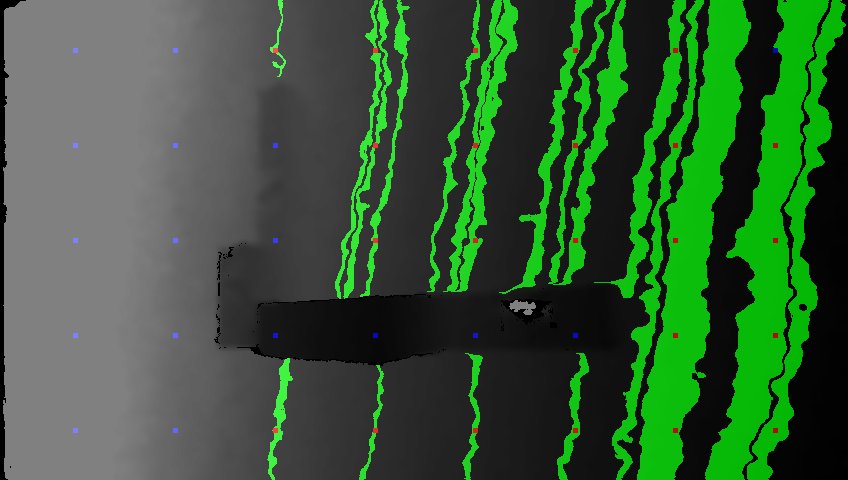
\includegraphics[width = \linewidth]{pictures/prob0001body_gnd.png}
    \caption[Expandování bodů odpovídajících zemi]{Expandování bodů odpovídajících zemi. Červenou barvou jsou znázorněny body, ze kterých probíhal algoritmus \ref{alg:floodfill}. Modré body byly podle výše uvedených kritérií vyřazeny a zeleně jsou znázorněny výsledné body reprezentující zem.}
    \label{fig:floodfill}
\end{figure}

Nyní vypočteme výšku každého bodu nad rovinou a prahováním této vzdálenosti přidělíme bodu hodnotu 0 až $k$, kde číslo reprezentuje očekávaný počet na sobě naskládaných cihel a $k$ maximální počet cihel, jenž může být na sebe naskládán. Vizualizace tohoto výsledku lze pozorvat na obrázku \ref{fig:height_map}

\begin{figure}
    \centering
    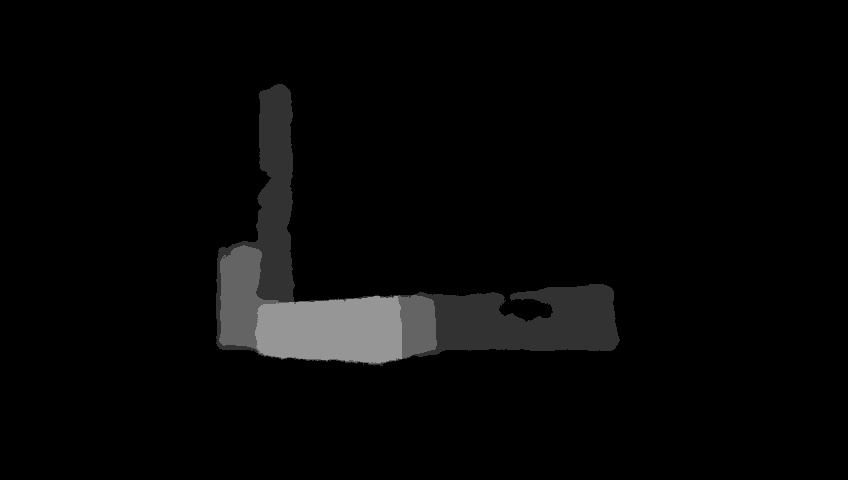
\includegraphics[width = \linewidth]{pictures/original_vrstva2_pic1.jpg}
    \caption{Vzdálenost bodů od roviny zobrazena jako počet na sobě lžících cihel}
    \label{fig:height_map}
\end{figure}

\subsection{Detekce normálového vektoru pomocí RANSAC}
\label{sec:plane_ransac}
Body jsou postupně prokládány rovinou pomocí RANSAC algoritmu, viz. \ref{sec:ransac}. Zde je potřeba správně určit kritérium, při jehož splnění budeme mít jistotu, že detekovaná plocha představuje zem. Pokud by algoritmus skončil po detekci plochy, v jejimž okolí leží nejvíce bodů, mohli bychom při velkém zastoupení kostek v obrazu dostat rovinu popisující horní stěnu těchto kostek. Jako terminační kritérium je tedy zvolena detekce dvou rovin a jejich následným porovnáním vybereme tu, která popisuje zemi.

\subsection{Přístup založený na změně výšky}
\label{sec:sobel_normal}
Velice populární postup při segmentaci obrazu je založen na porovnávání normálového vektoru v bodech obrazu, viz sekce \ref{sec:normal_methods}. Normálový vektor je vypočten pro každý bod obrazu a následně jsou body, jejichž normálový vektor má podobný směr, popřípadě i velikost, sloučeny do větších celků. V našem případě je vrchní stěna cihly paralelní se zemí a má tedy stejný normálový vektor. Nachází se však v jiné výšce. Pomocí výpočtu gradientu, který budeme realizovat užitím Sobelova operátoru aplikovaného na výšku bodů, spočítáme derivaci výšky. Ta by měla být nejvyšší v oblasti přechodu země - cihla. Následně pak sloučíme body s hodnotou gradientu výšky, která se liší v rámci skupiny maximálně o $\delta$. K tomu bylo využito upraveného Connected-component labeling (CCL) algoritmu. 

Tato metoda při správném odladění parametru $\delta$ pro danou scénu dosahuje velmi dobrých výsledků. Problémem je však robustnost. Hodnoty parametru $\delta$ fungující na cihly v blízkosti kamery nefungují na cihly ve vzdálenosti řádově 2\,$m$ a více a naopak. Toto je způsobeno jednak šumem kamery, který podle rovnice \ref{error_stereo} roste kvadraticky, a zejména pak zkreslením vzdálenější hrany cihly kamerou, viz. obrázek \ref{fig:point_cloud_grad}. Kamera zde špatně nachází stereo páry a generuje mračna bodů, která ve skutečnosti neexistují. Ty zmírňují přechod cihla-zem a snižují tak hodnotu gradientu. 
\begin{figure}
    \centering
    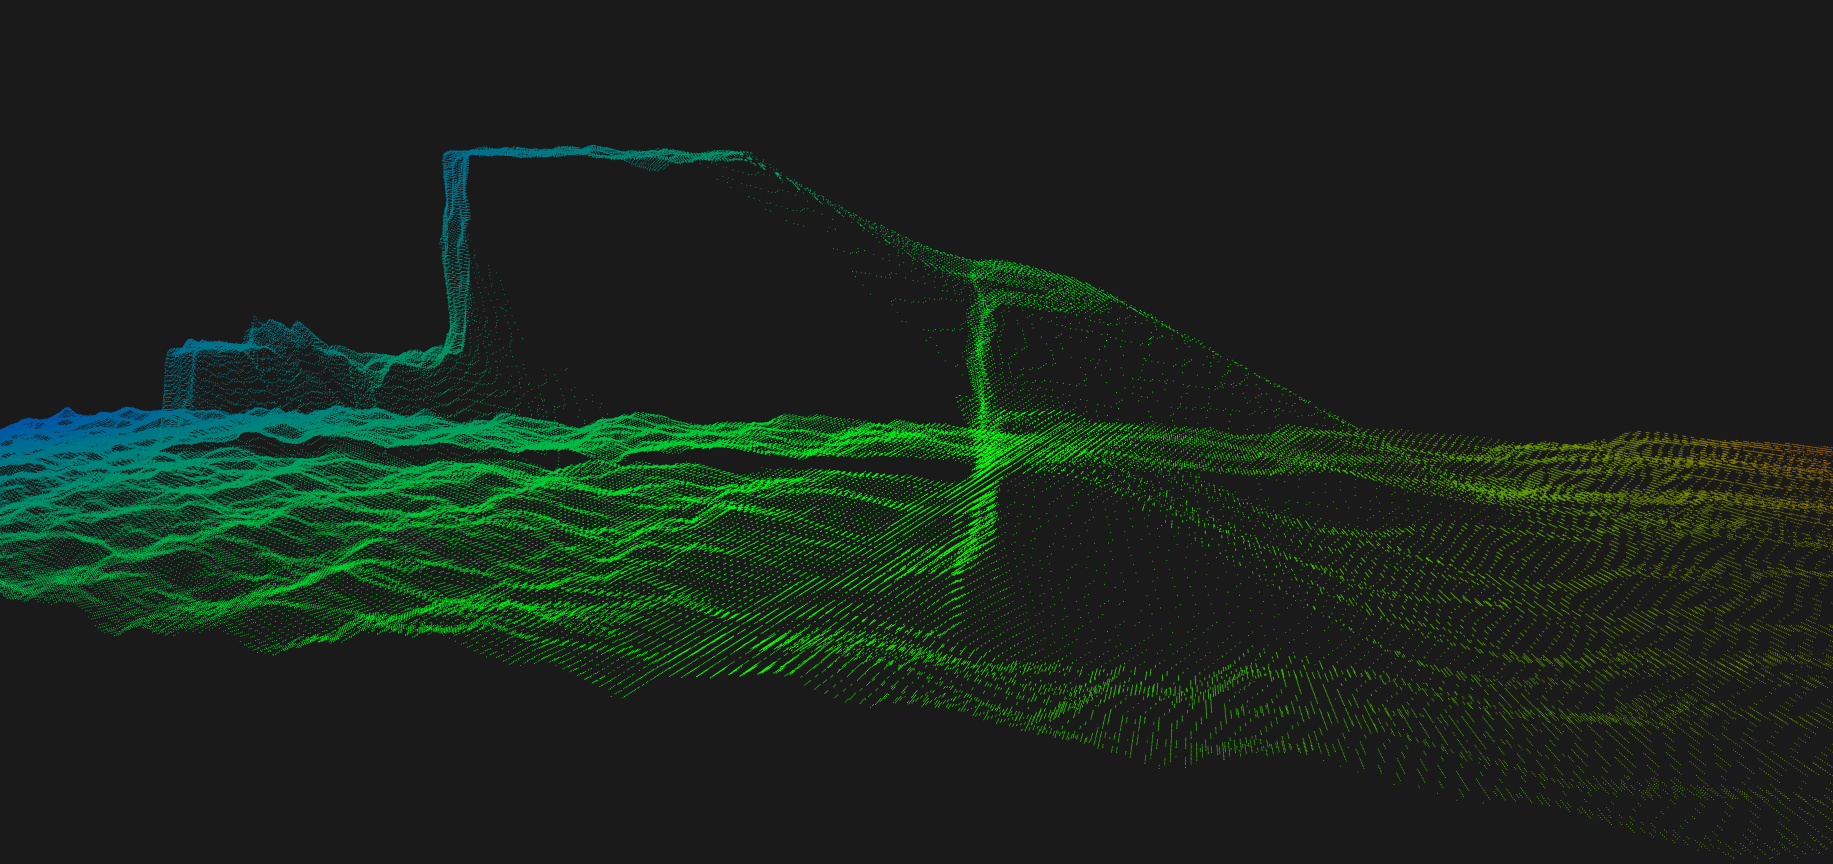
\includegraphics[width = \linewidth]{pictures/pc_crop.png}
    \caption[Výstup kamery]{Výstup kamery - mračno bodů zobrazující skupinu cihel. V pravé části je vidět zkreslení hrany způsobující problém při segmentaci}
    \label{fig:point_cloud_grad}
\end{figure}

%\begin{figure}
    %\centering
    %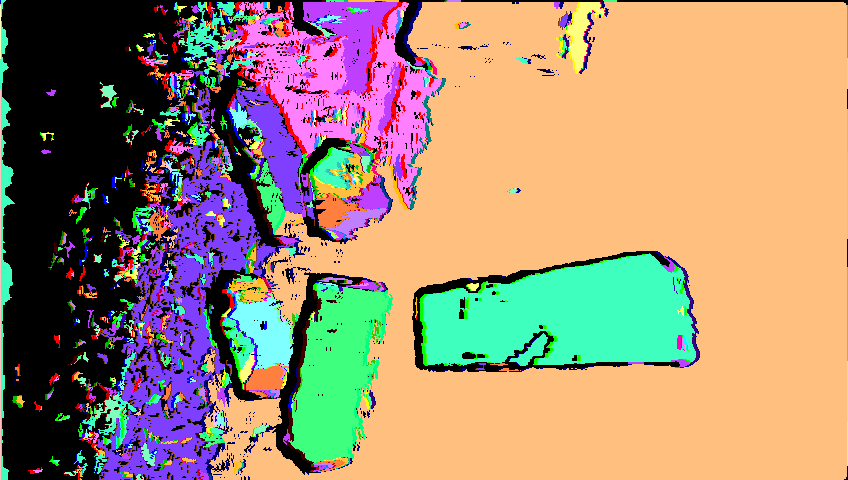
\includegraphics[width = \linewidth]{pictures/obr10_grad.png}
    %\caption{Výsledek segmentace obrazu podle velikosti derivace výšky.}
    %\label{fig:sobel_segment}
%\end{figure}

\section{Detekce objektů ze segmentovaného obrazu}
Stejně jako při segmentaci obrazu, tak i zde bylo vyzkoušeno několik algoritmů. Některé z nich byly nastaveny na detekci za zjednodušujících podmínek a nabízí tak nižší výpočetní náročnost při stejné přesnosti detekce. 
Vstupem všech prezentovaných algoritmů bude segmentovaný obraz $X$, jako je například obrázek \ref{fig:height_map}. Tedy pro každý bod obrazu \tl{p} známe jeho atribut $L(\mathbf{p})$, který reprezentuje počet na sobě naskládaných cihel v bodě \tl{p}. % Tedy vstupem je presketivně deformovaný púdorys jednotlivých cihel.

\subsection{Detekce pomocí nejmenšího ohraničujícího obdélníku}
\label{sec:bounding_rect}
V tomto algoritmu předpokládáme, že cihly se navzájem nedotýkají, popřípadě se dotýkají pouze po celé délce navzájem si odpovídajících stěn.

Principem tohoto algoritmu je transformace jednotlivých vrstev tak, aby jejich půdorys nebyl zkreslený prespektivní transformací. Následně je z půdorysu vrstvy určena poloha kostky v dané vrstvě.

Chceme-li určit půdorys $n$-té vrstvy cihel, pak je k tomu potřeba znát půdorysy vrstev $n,...,m$, kde $m$ je nejvyšší vrstva cihel v obrazu. 
Obraz $X$ je nejprve prahován podle $L$, viz sekce \ref{subsection:segmentation}, kde spodním limitem prahování je $n$. Na prahovaný obraz je použita morfologická operace otevření, viz sekce \ref{sec:morphology}. Pomocí této operace je obraz vyfiltrován a jsou odstraněny body představující šum, viz obrázek \ref{fig:morfology_open}. Následně jsou nalezeny vnější obrysy  shluků cihel\footnote{Shlukem cihel se myslí skupina cihel, které jsou spojeny dotekem.} pomocí Suzukiho algoritmu \cite{suzuki1985topological}, kde jsme využili již implementovaného programu v knihovně OpenCV\cite{opencv_library}.

\begin{figure}
    \centering
    \begin{subfigure}{0.4\textwidth}
      \centering
      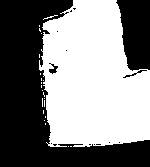
\includegraphics[width=0.93\linewidth]{pictures/before_open.png}
      \caption{Obraz před filtrací}
      \label{subfig:pic_close}
    \end{subfigure}
    \begin{subfigure}{0.39\textwidth}
      \centering
      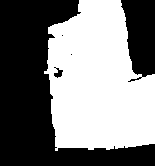
\includegraphics[width=0.99\linewidth]{pictures/after_open.png}
      \caption{Obraz po filtraci}
      \label{subfig:pic_open}
    \end{subfigure}
    \caption{Filtrování obrazu pomocí morgologické oprace otevření}
    \label{fig:morfology_open}
\end{figure}
Pomocí průměrového filtru jsou vyhlazena data reprezentujících obrys shluku cihel, resp. jejich výška. Poté je obrys aproximován konvexním obalem, čímž se zmenší počet bodů, kterými je daný shluk popisován.

Obraz horní stěny kvádru nepodléhá prespektivnímu zkreslení, je-li horní stěna kolmá na optickou osu kamery. Tedy normálový vektor reprezentující horní stěnu kvádru musí být rovnoběžný s optickou osou kamery. Normálový vektor horní stěny kvádru ležícího na zemi je stejný s normálovým vektorem \tl{n} země, který byl určen v sekci \ref{sec:normal_est}. Natočení země vůči kameře je vnější parametr kamery. Body obrazu můžeme tedy transformovat do jejich projekce na rovinu země pomocí upraveného vzorce \ref{eq:world_to_img} jako %\unsure{Bod \tl{x} bude vyjádřen v homogenních souřadnicích a bude mít tedy tvar x,y,z,1 ...mohu rovnici dole zapsat takto? jedná se o korektní převedení rovnice \ref{eq:world_to_img}, nebo musím explicitně vyjádřit \tl{x}?  Myslím, že můžete použít již zavedené vzorce a jen na ně odkázat.}
\begin{align}
    \mathbf{x} = \begin{bmatrix} \mathbf{I} \\ 0 \end{bmatrix} \mathbf{K}^{-1} \mathbf{R}^{-1}\mathbf{x}_p, \label{eq:pic_to_world}
\end{align}
kde \tl{R} je matice určená pomocí Rodriguezova vzorce \ref{Rodriguez}. Úhel $\theta$ mezi optickou osou a normálovým vektorem byl určen pomocí vztahu \ref{eq:angle_rogrig} a vektor $\tilde{\mathbf{u}}$, kolem které rotace probíhá, pomocí vztahu \ref{eq:vector_rogrig}. Po provedení této transformace dostaneme body, které představují konvexní obal, zbavené prespektivního zkreslení.

Následně je nalezen nejmenší obdélník, který opisuje tyto body, viz sekce \ref{sec:nejmenší_obdélník}. Tímto dostaneme řešení ve světovém souřadném systému. Obdélník je plně popsán svými vrcholy. Na tyto vrcholy aplikujeme transformaci \ref{eq:world_to_img}, kde matice \tl{R} je transpnovaná matice \tl{R} určena výše. Dostaneme body v obraze, které odpovídají ohraničujícímu obdélníku po aplikování prespektivního zkreslení. Jelikož výška $h$ každé cihly je stejná a ze zadání známá, je možné nalezené vrcholy posunout o $h$ a získat tak zbylé vrcholy cihly. Tímto způsobem bude ohraničující kvádr obsahovat i prostorovou informaci.

Výše uvedený postup je proveden pro každý obrys odpovídající skupině kostek a následně pro každé patro. Výsledek algoritmu je vidět na obrázku \ref{fig:bb_clasic}

\begin{figure}
    \centering
    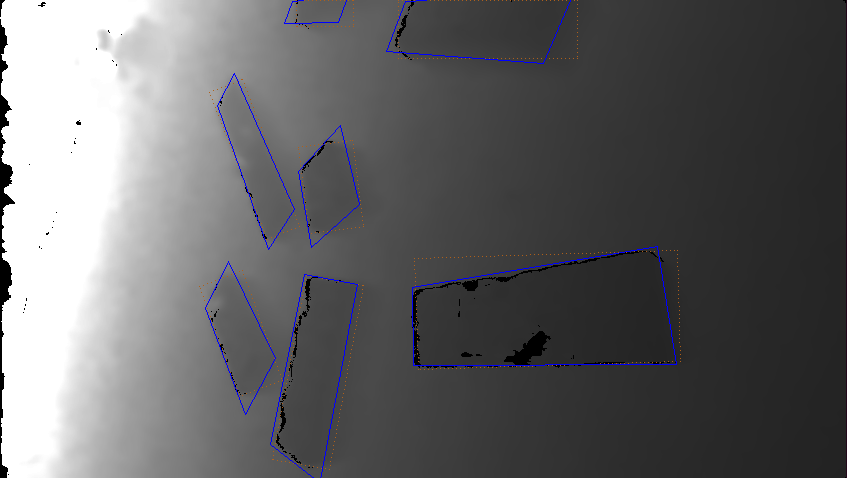
\includegraphics[width = 0.7\linewidth]{pictures/detekce_bb.png}
    \caption[Příklad detekce cihel z hloubkových dat]{Příklad detekce cihel z hloubkových dat. Modře ohraničující obdélník po odstranění prespektivního zkreslení, hnědě ohraničující obdélník u kterého není bráno v potaz prespektivní zkreslení}
    \label{fig:bb_clasic}
\end{figure}

\subsection{Detekce pomocí RANSAC}
\label{sec:ransac_det}
Postup popsaný v sekci \ref{sec:bounding_rect} funguje pouze za zjednodušujících předpokladů a navíc jeho přesnost značně klesá při nesprávném generování stereo párů, jak je vidět na obrázku \ref{fig:point_cloud_grad}. Tato metoda funguje pro všechna natočení cihel a je i velice robustní.
\begin{figure}
    \centering
    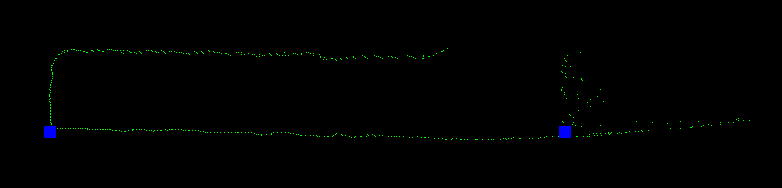
\includegraphics[width = \linewidth]{pictures/crop_ransac_rot.png}
    \caption{Detekce kratších hran cihly.}
    \label{fig:RANSAC_line_short}
\end{figure}
\begin{figure}
    \centering
    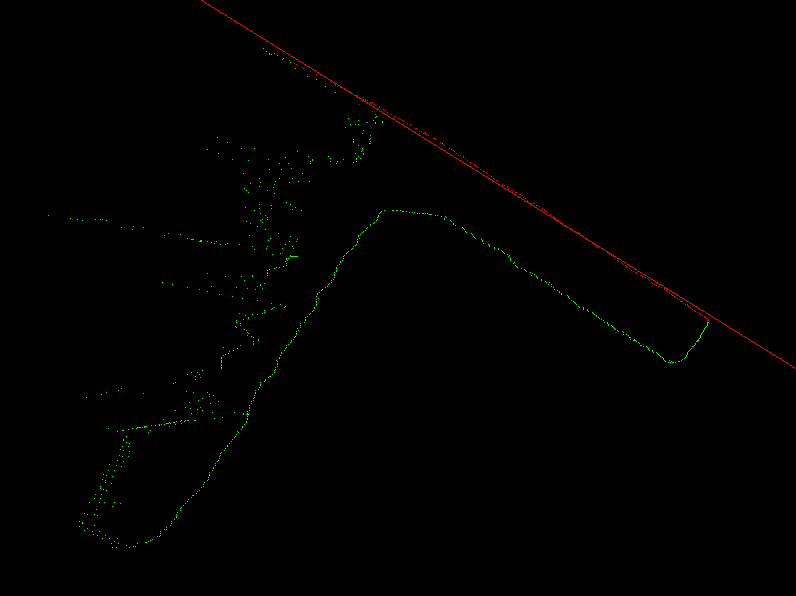
\includegraphics[width = \linewidth]{pictures/ransac_rect_fit1.png}
    \caption{Detekce delší hrany cihly pomocí RANSAC algoritmu}
    \label{fig:RANSAC_line}
\end{figure}

Začneme obdobně jako v sekci \ref{sec:bounding_rect} transformací bodů představující obrys pomocí vztahu \ref{eq:pic_to_world}. Mezi body představující prespektivně nezkreslený obrys najdeme pomocí RANSAC přímku $p_1$. Ta odpovídá jedné z delších stěn cihly, viz. obrázek \ref{fig:RANSAC_line}. Následně je opět použit algoritmus RANSAC a mezi zbylými body je nalezena přímka $p_2$ rovnoběžná s $p_1$. Tímto dostaneme obě protější stěny cihly. Hledání zbylých dvou kratších stěn je pomocí RANSAC algoritmu nerealizovatelné, jelikož tyto stěny jsou tvořeny malým počtem bodů. Pokud je obraz zašuměn, pak není možné najít přímky odpovídající těmto krátkým stěnám.

Kratší stěny cihly tedy určíme následovně. Vybereme množinu bodů, které leží mezi přímkami $p_1$ a $p_2$. Poté tyto body promítneme na přímku $p_1$. Výpočet numericky zjednodušíme otočením bodů a přímek o $\theta$, což je úhel sevřený přímkou $p_1$ a osou $x$. Projekce na přímku $p_1$ se tedy stane vyčtením $x$-ové souřadnice každého bodu.

Následně je pro každý bod $\mathbf{x} \in p_1$ určen počet bodů promítnutých do okolí o velikosti $\epsilon$ a jsou vybrány dva body s nejvyšší hodnotou. Tyto body jsou ilustrovány na obrázku \ref{fig:RANSAC_line_short} modrou barvou. Těmito body prochází přímky $p_3$ a $p_4$, které jsou kolmé na $p_1$, popřípadě $p_2$, a představují zbylé dvě stěny hledaného obdélníku. Vrcholy obdélníku $r$ pak určíme jako průsečíky přímek $p$.

Nyní se z bodů představující obrys shluku cihel odečtou ty, které popisují obdélník $r$. Pokud počet zbývajících bodů obrysu je větší než předem určený limit, pak se proces počínaje hledáním přímky $p_1$ opakuje.

Ve chvíli kdy jsou nalezeny všechny obdélníky a nezbývají již žádné volné body, jsou tyto obdélníky, stejně jako v sekci \ref{sec:bounding_rect}, pomocí svých vrcholů transformovány zpět do obrazu a celý postup se opakuje pro další shluky a vrstvy cihel.
\begin{figure}
    \centering
    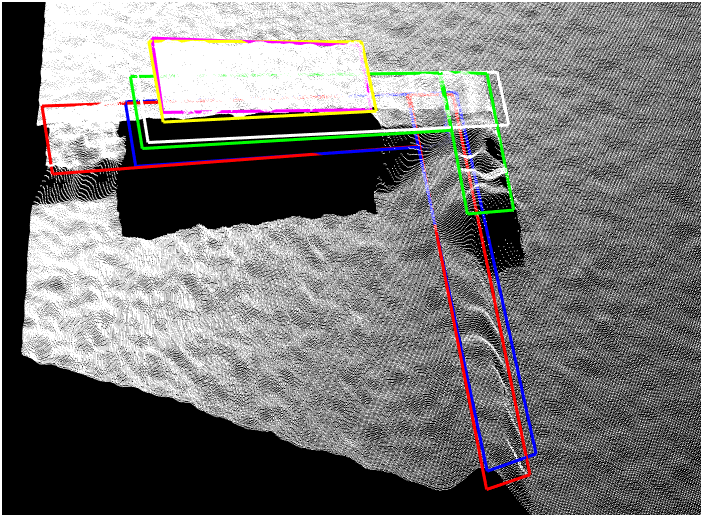
\includegraphics[width = \linewidth]{pictures/upraveno_3rdlayaer.png}
    \caption[Výsledek detekce cihel zanesený v mračně bodů]{Výsledek detekce cihel zanesený v mračně bodů. Červenou, bílou a řůžovou barvou jsou znázorněny manuálně zanesené polohy cihel.}
    \label{fig:all_layers_det}
\end{figure}




%\end{figure}


\chapter{Výsledky}
\label{sec:výsledky}
%\todo[inline]{Porovnání jednotlivých výsledků, přesnost + časová náročnost}
%Za účelem vyhodnočení výsledků bylo ručně 
\section{Označení polohy cihel v mračnech bodů}
Za účelem vyhodnocení přesnosti algoritmů prezentovaných v sekci \ref{sec:navrzene_reseni}, jsme ručně zanesli polohu jednotlivých cihel do mračen bodů. Vzhledem k nedostupnosti nekomerčních softwarů umožňujících manuální označování v mračnech bodů jsme vytvořili vlastní aplikaci v prostředí Point Cloud Library (PCL) \cite{pcl}. Ta pro každé mračno bodů kombinací RANSAC a PCA algoritmu přesně určí rovinu reprezentující zem. Následně jsou odstraněny body reprezentující zem a do zbylých bodů jsme ručně zanesli polohu první vrstvy cihel. Tento postup se opakuje pro každé patro zdi, jak je možné vidět na obrázku \ref{fig:labler}.
Tímto způsobem jsme označili 20 náhodně vybraných obrázků obsahujících nedotýkající se cihly a 15 obrázků, na kterých cihly tovří složitější struktury. Poloha všech cihel je nakonec uložena do textového souboru, kde je každá cihla reprezentována čtyřmi body v euklidovském prostoru a číslem označujícím vrstvu, ve které se nachází.
\begin{figure}[h]
    \centering
    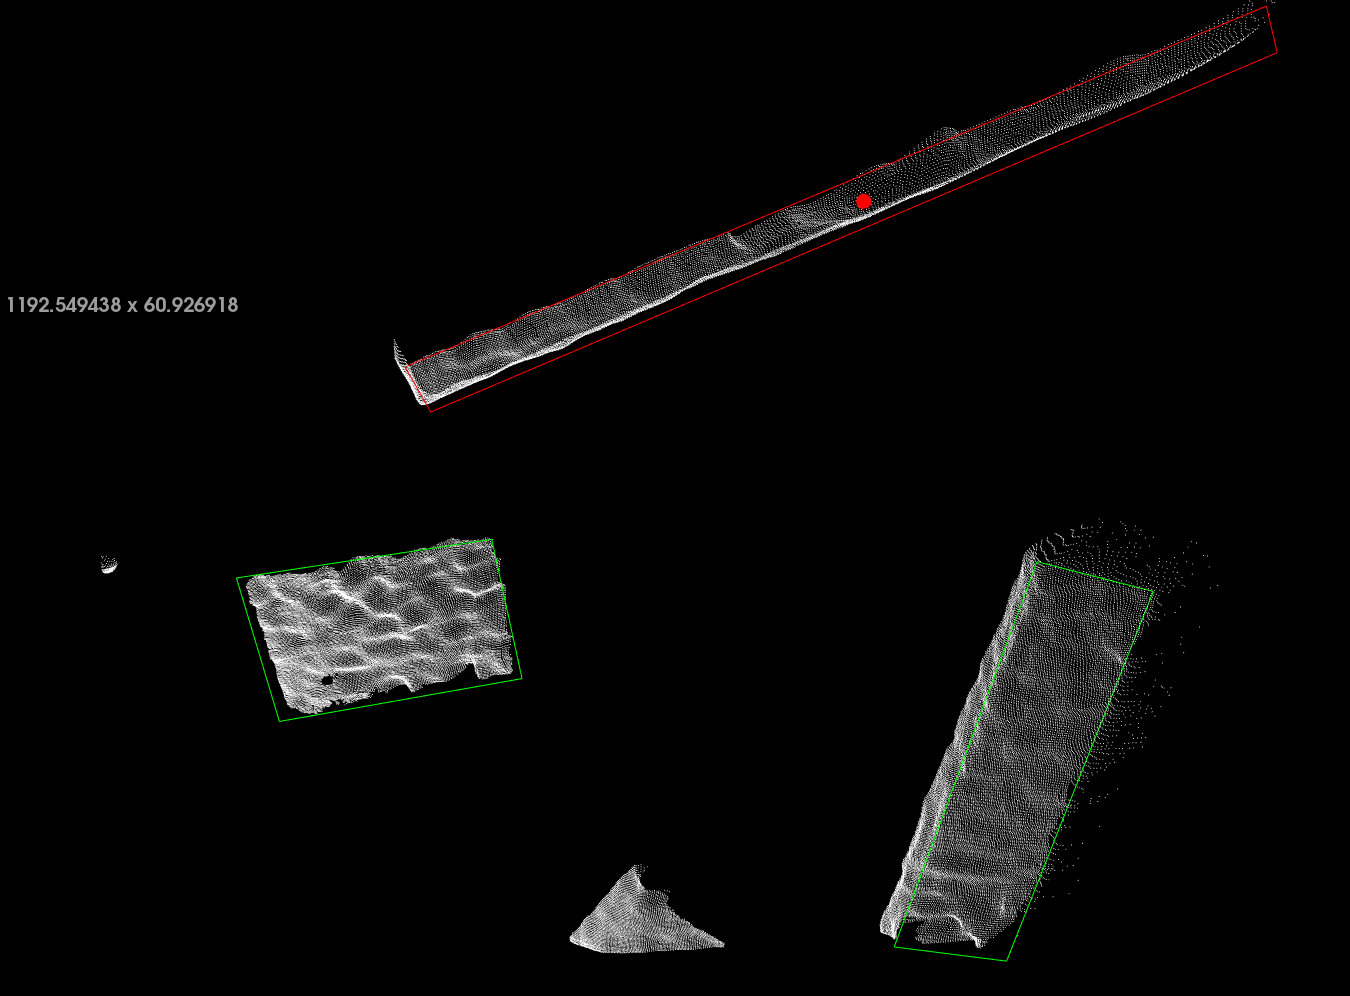
\includegraphics[width = 0.8\linewidth]{pictures/labelr.png}
    \caption{Prostředí aplikace pro označení pozice cihel}
    \label{fig:labler}
\end{figure}

\section{Vyhodnocovací kritéria}
Úspěšnost detekce je hodnocena podle časové náročnosti daného programu a přesnosti detekce jednotlivých cihel. Při vyhodnocení přesnosti detekce hodnotíme pouze přesnost umístění horní stěny cihly, jelikož ostatní parametry je možné dopočítat ze znalosti normálového vektoru země.

Nechť $C$ je mračno bodů, pro které bylo manuálně zaznamenáno 
$m$ poloh  obdélníků $L_i$, které reprezuntují polohu cihel. Pokud náš program na detekci cihel vrátí množinu obdélníků $S_1 ... S_n$, pak se přesnost $p(C)$ určí následovně.
\begin{align}
    A(L) = \sum_{i=1}^{i = m}|\rectangle L_i| \quad A(S) = \sum_{i=1}^{i = n}|\rectangle S_i|, \quad I = \sum_{i = 1}^{i = n} \sum_{j = 1}^{j=m} | \rectangle S_i \cup \rectangle L_j | \label{eq:flat} \\
    \text{TP} = I, \quad \text{FP} = A(S) - I, \quad \text{FN} = A(L) - I \\
    p = \frac{\text{TP}}{\text{TP} + \text{FN} + \text{FP}} \label{eq:accuracy}
\end{align}
V rovnici \ref{eq:flat} jsme symbolem $|\rectangle L_i|$ označili plochu určenou obdélníkem $L_i$.  
Časová náročnost programu je určena měřením času běhu programu na jednom jádře procesoru Intel\textregistered{} Core\textsuperscript{TM} i5-7200U, který pracuje s frekvencí 2,5$\,$GHz v normálním módu a s frekvencí 3,1$\,$GHz v turbo módu.

\section{Určení normálového vektoru}
\label{sec:res_normal}
Přesnost určení normálového vektoru jsme vyhodnotili na základě přesnosti detekce objektů, jelikož tato detekce silně závisí na přesnosti určení normálového vektoru. Jedná se navíc o jediné relevantní kritérium, podle kterého můžeme přesnost určit.

Výsledky algoritmu prezentovaného v sekci \ref{sec:sobel_normal} nebudeme vyhodnocovat, jelikož nebylo možné nastavit parametry algoritmu tak, aby detekoval normálový vektor země při různé vzdálenosti kamery od obrazu.

\begin{figure}
    \centering
    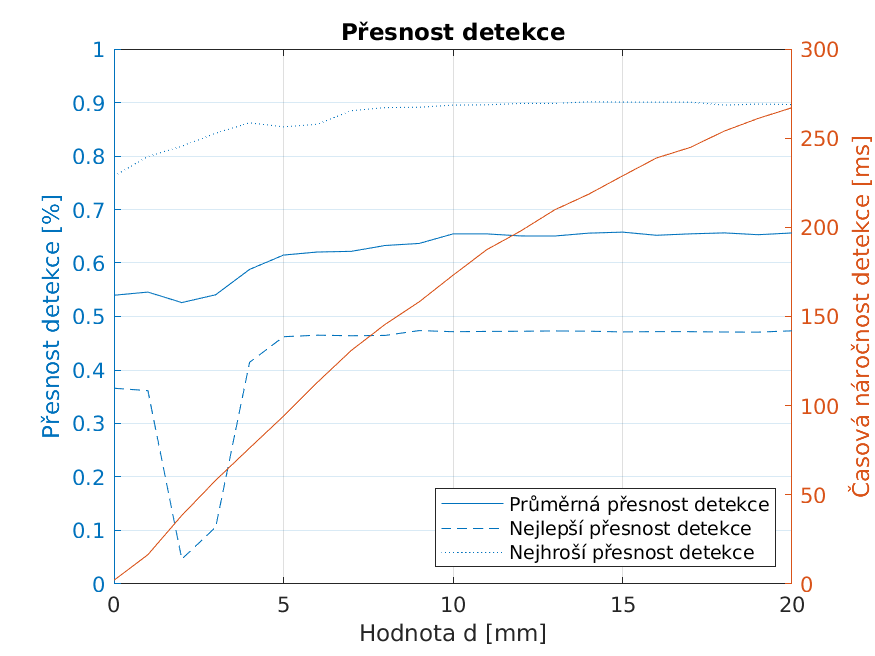
\includegraphics[width =0.8\linewidth]{pictures/normal_acc.png}
    \caption{Přesnost detekce v závislosti na parametru $\delta$}
    \label{fig:delta_detekce_normaly}
\end{figure}

Přesnost a doba průběhu programu, který byl popsán v sekci \ref{subsec:height}, záleží zejména na velikosti parametru $\delta$, který určuje množství bodů, kterými bude v druhém kroku programu proložena rovina algoritmem PCA. Závislost přesnosti na časové náročnosti programu můžeme pozorovat na grafu \ref{fig:delta_detekce_normaly}, kde detekce byla provedena algoritmem popsaným v sekci \ref{sec:bounding_rect}. RANSAC algoritmus \ref{sec:ransac_det} vykazoval podobnou tendenci přesnosti detekce v závislosti na parametru $\delta$ a není tedy uváděn.

Chování algoritmu \ref{sec:plane_ransac} závisí především na dvou parametrech a to maximálním počtu iterací $n$ a vzdálenosti $\epsilon$ od modelu, ve které se musí nacházet bod, aby byl uvažován součástí modelu. Závislost přesnosti a časové náročnosti na $\epsilon$ je vidět na grafu \ref{fig:plane_ransac}, kde  byl algoritmus testován při neomezeném počtu iterací. Můžeme pozorovat, že algoritmus dosahuje nejlepších výsledků při $\epsilon = 60\,mm - 100\,mm$.

\begin{figure}
  \centering
  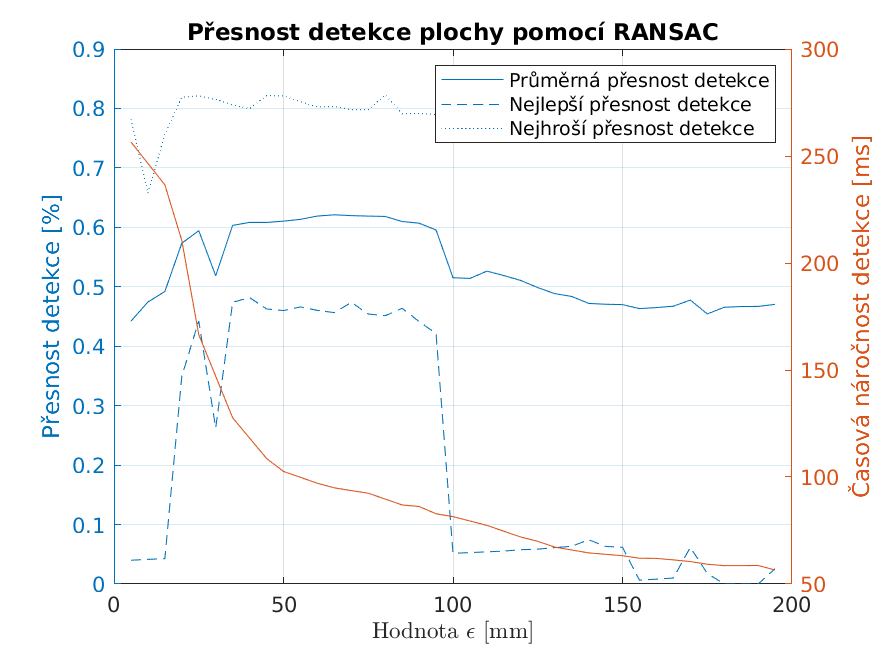
\includegraphics[width=0.8\linewidth]{pictures/plane_ransac.png}
  %\caption{Závislost přesnosti na $\epsilon$}
  \label{subfig:epsilon}
  \caption{Přesnost RANSAC algoritmu pro detekci plochy v závislosti na $\epsilon$}
\label{fig:plane_ransac}
\end{figure}

Pro hodnotu parametru $\epsilon = 80\,mm$ jsme provedli test závislosti přesnosti na maximálním počtu iterací. Výsledky na obrázku \ref{fig:ransac_max_iter} jsou průměrem pěti průběhů testu, jelikož RANSAC je nedeterministický algoritmus a jeho výsledky se v každém běhu mohou výrazně lišit. Z grafu je vidět, že maximální přesnost je vždy dosažena nejpozději po 12-ti iteracích. Časová náročnost stále stoupá, jelikož jsme využili již implementovaného RANSAC algoritmu v knihovně PCL \cite{pcl}, který byl lépe optimalizovan než naše implementace. Nenabízí však možnost ukončení algoritmu, pokud pro daný počet bodů $\mathbf{p}_i$ platí $|\mathbf{p}_i - \mathbf{m}| < \epsilon$, kde \tl{m} je bod modelu, který je nejblíže bodu $\mathbf{p}_i$.

\begin{figure}
    \centering
    \begin{subfigure}{0.5\textwidth}
      \centering
      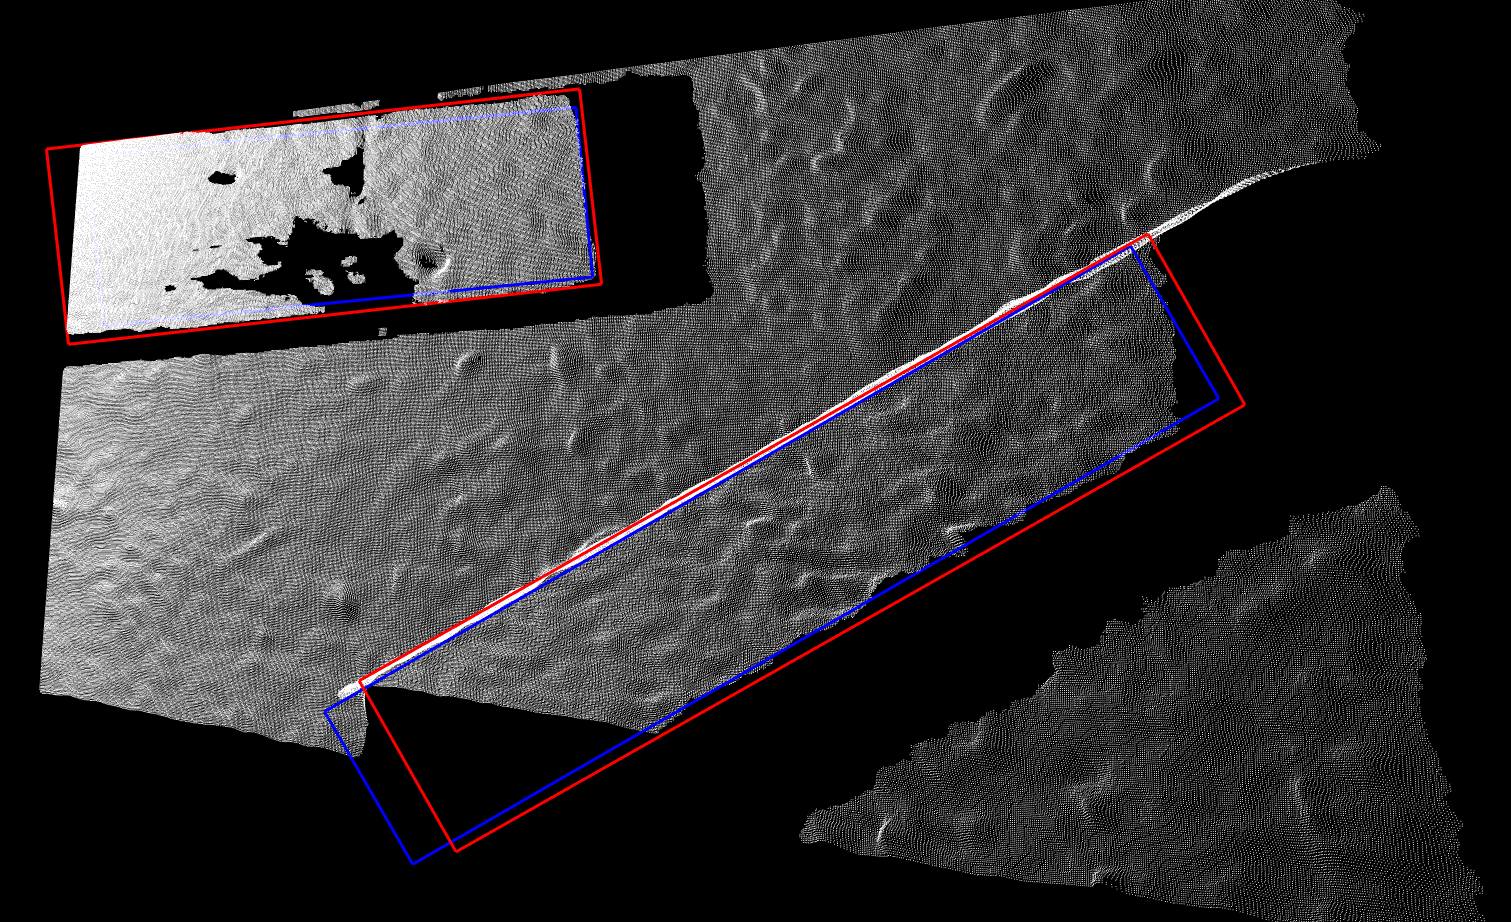
\includegraphics[width=0.99\linewidth]{pictures/res_det_good.png}
      \caption{Nejlepší detekce v datasetu}
      \label{subfig:object_det_good}
    \end{subfigure}
    \begin{subfigure}{0.49\textwidth}
      \centering
      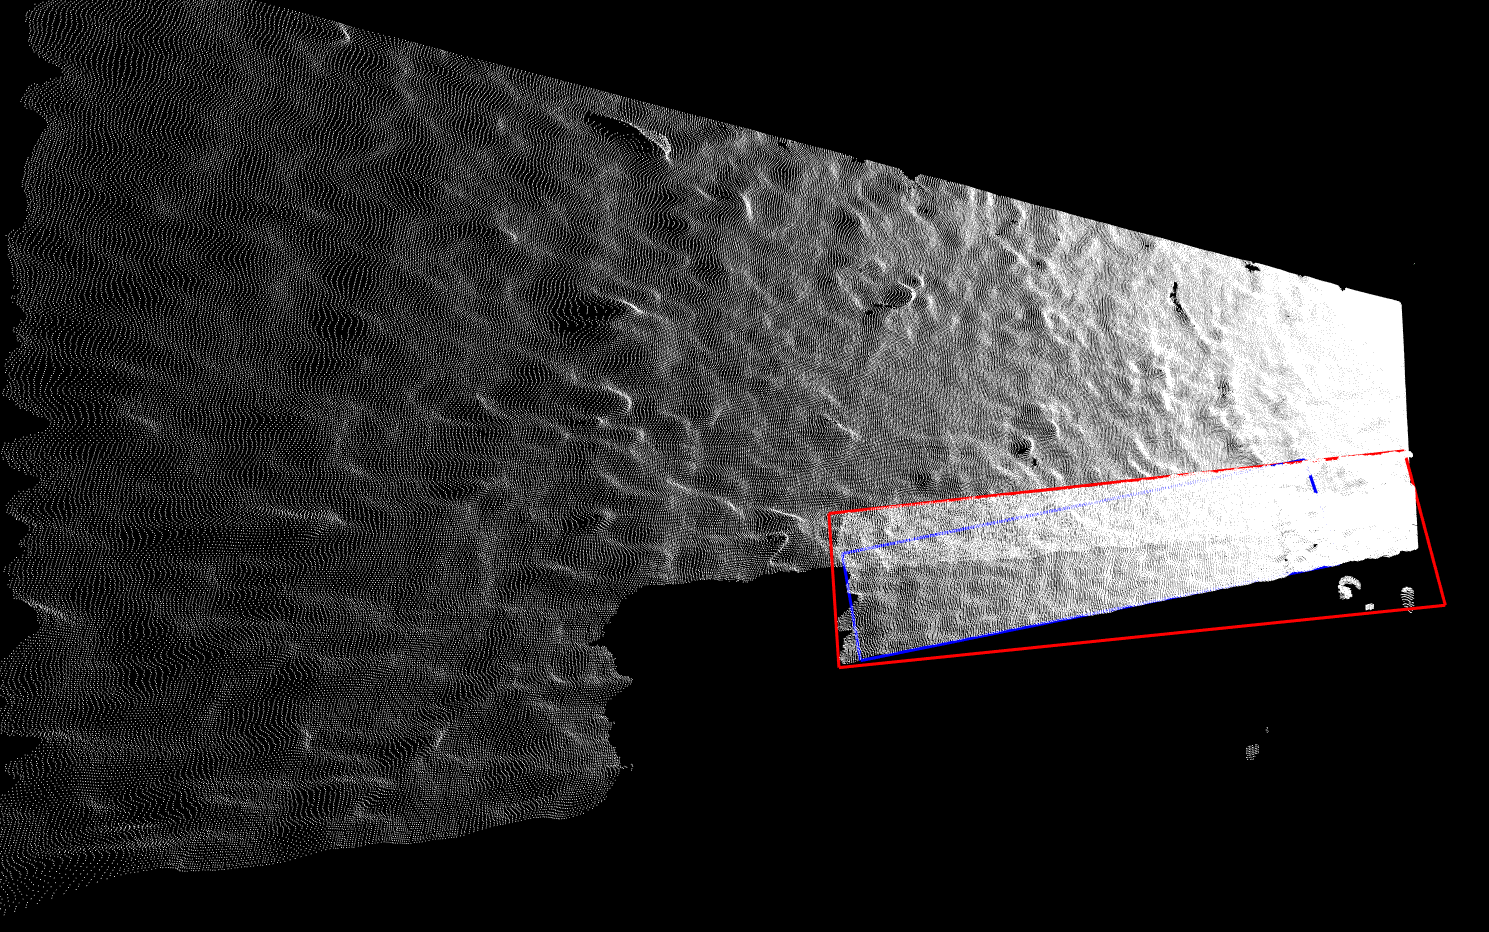
\includegraphics[width=0.99\linewidth]{pictures/res_det_bad.png}
      \caption{Nejhroší detekce v datasetu}
      \label{subfig:object_det_bad}
    \end{subfigure}
    \caption{Ilustrace výsledků detekce cihel}
    \label{fig:object_det_res}
\end{figure}
\begin{figure}
    \centering
    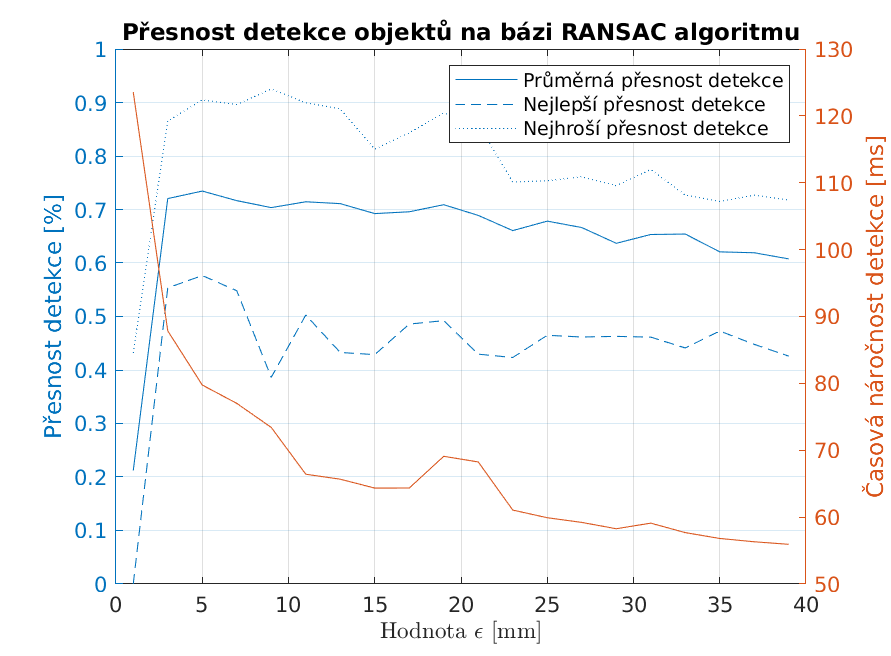
\includegraphics[width = \linewidth]{pictures/ransac_obj_det.png}
    \caption{}
    \label{fig:ransac_obj_det}
\end{figure}

Po detekci normálového vektoru následuje sémantická segmentace obrazu. Tato segmentace probíhá pro všechny metody detekce prahováním vzdálenosti jednotlivých bodů od nelezené plochy reprezuntující zem. Jedná se o deterministický algoritmus, který proběhne v čase $62\,ms$.

\section{Detekce objektů}
\subsection{Nedotýkající se cihly}
V této sekci budou všechny programy testovány na datasetu, kde se jednotlivé cihly vzájemně nedotýkají.

Přesnost algoritmu, který byl popsáného v sekci \ref{sec:bounding_rect} je vidět na grafech \ref{fig:delta_detekce_normaly}, \ref{fig:plane_ransac}, \ref{fig:ransac_max_iter}. Doba průběhu algoritmu závisí na počtu cihel, které se nachází ve scéně. Průměrně je detekce provedena v čase $872\,ns$ a nejpomalejší detekce v testovaném datasetu byla provedena za čas $978\,ns$.

Algoritmus pro detekci založený na bázi RANSAC algoritmu popsaný v sekci \ref{sec:ransac_det} si dynamicky určuje maximální počet iterací v závislosti na počtu bodů, které tvoří obrys skupiny kostek. Chování tohoto algoritmu je tedy určeno parametrem $\epsilon$, jehož význam je stejný jako v sekci \ref{sec:res_normal}. Přesnost detekce a časová náročnost v závislosti na $\epsilon$ je vidět na obrázku \ref{fig:ransac_obj_det}. Normálový vektor země, který je pro detekci potřeba, byl určen pomocí modifikovaného PCA algoritmu, který byl popsan v sekci \ref{subsec:height}.


Výsledky detekce můžeme pozorovat na obrázku \ref{fig:object_det_res}, kde modrou barvou je značen výsledek programu a červeně manuálně zanesená poloha cihel. Z obrázku \ref{subfig:object_det_good} je vidět, že detekce probíhá velice přesně a chyba algoritmu může být způsobena nepřesností při označování skutečných poloh cihel. Dokonce i nejhorší detekce v celém datasetu, která je na obrázku \ref{subfig:object_det_bad}, správně nalezne nacházející se cihlu, pouze špatně odhadne její natočení a velikost.

 
\subsection{Dotýkající se cihly}
Jediný algoritmus schopný detekce dotýkajících se cihel je popsán v sekci \ref{sec:ransac_det}. Jeho výsledky na datasetu s nedotýkajícími se cihlami lze pozorovat na obrázku \ref{fig:ransac_obj_det}. Pro parametr $\epsilon = 12\,mm$ dostaneme na datasetu, který obsahuje pouze složitější struktury cihel, následující výsledky.
\begin{itemize}
    \item Průměrná úspěšnost detekce $68,24\,\%$
    \item Nejlépe klasifikované mračno bodů $84,3\,\%$
    \item Nejhůře klasifikované mračno bodů $39,7\,\%$
    \item Průměrná časová náročnost $78,8\,ms$
\end{itemize}
Algoritmus tedy dosahuje podobných výsledků, jako při detekci nedotýkajících se cihel, pouze v horším časem. Příklad úspěšné detekce je vidět na obrázku \ref{fig:all_layers_det}
\section{Shrnutí výsledků}
V této sekci srovnáme výsledky kombinací jednotlivých algoritmů. Součástí každého z nich je prahování bodů podle vzdálenosti od roviny, které trvá $62\,ms$.

V tabulce \ref{tab:vysledky} jsou použity následující zkratky RANSAC - detekce plochy pomocí ransac algoritmu, kde $li$ a $hi$ značí nízký a vysoký počet maximálních iterací. Jako PCA je označen algoritmus pro detekci plochy pospaný v sekci \ref{subsec:height}, kde $m$ a $v$ značí nízkou a vysokou hodnoty parametru $d$. Označením RANSAC-det je myšlen algoritmus popsaný v sekci \ref{sec:ransac_det}.
\begin{table}[h]
    \centering
    \begin{tabular}{|l|c|c|c|c|c|c|} \hline
        algoritmus &  přesnost [\%]& čas [ms]\\ \hline
        RANSAC-$li$ a Nejmenší ohraničující odbélník & 43,2 & 108 \\ \hline
        RANSAC-$hi$ a Nejmenší ohraničující obdélník & 61,3 & 143 \\ \hline
        PCA-$n$ a Nejmenší ohraničující obdélníku & 57,5 & 148 \\ \hline 
        PCA-$v$ a Nejmenší ohraničující obdélník & 65,2 & 243 \\ \hline
        RANSAC-$li$ a RANSAC-det & 58,4 & 182 \\ \hline
        RANSAC-$hi$ a RANSAC-det & 68,7 & 217 \\ \hline
        PCA-$n$ a RANSAC-det & 63,1 & 223 \\ \hline 
        PCA-$v$ a RANSAC-det & 70,8 & 328 \\ \hline
        PCA-$v$ a RANSAC-det - složité objekty & 68,24 & 341 \\ \hline
    \end{tabular}
    \caption{Porovnání výsledků jednotlivých algoritmů}
    \label{tab:vysledky}
\end{table}
\begin{figure}
    \centering
    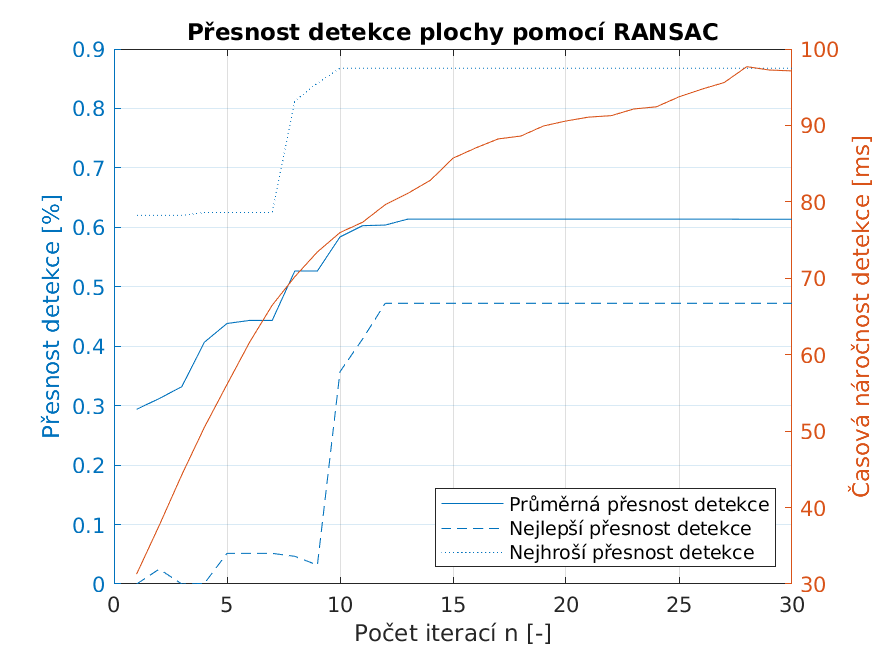
\includegraphics[width =0.8\linewidth]{pictures/plane_ransac_iter.png}
    \caption{Přesnost RANSAC algoritmu pro detekci plochy v závislosti na $n$}
    \label{fig:ransac_max_iter}
\end{figure}
\chapter{Závěr}
\label{sec:závěr}
V této práci jsme se seznámili s principem funkce stereokamery a metodami detekce z hloubkových dat. Těchto znalostí jsme následně využili k navržení vlastních postupů pro detekci na zemi ležících cihel. Vstupními informacemi našeho programu byla data ze stereokamery Intel\textregistered{} RealSense$^{TM}$. Následně byly tyto postupy implementovány v jazyce \CC{} s využitím knihoven OpenCV\cite{opencv_library} a PCL\cite{pcl}.

Nejpřesnější z námi prezentovaných postupů je schopn detekovat objekty s úspěšností 70,8\,\%. Je však omezen na bloky cihel, mezi kterými nedochází k vzájemnému doteku, popřípadě se bloky mohou dotýkat po celé délce odpovídající stěny.

Tento program byl dále rozšířen, aby byl schopen detekce cihel nacházejících se ve složitějších strukturách, jako je třeba zeď tvořící roh, viz obrázek \ref{fig:all_layers_det}. Tyto ztěžující podmínky mají pouze minimální vliv na výsledky programu. Detekce je provedena se ztrátou přesnosti 2,56\,\% a pouze o 13\,ms pomaleji.

Prezentované výsledky byly získány na datasetu, který byl pořízen člověkem držícím Intel\textregistered{}  RealSense$^{TM}$ kameru. Toto zapříčinilo menší úhel mezi rovinou země a optickou osou kamery. Kvůli tomu je na všech datech pozorovatelné velké prespektivní zkreslení. Předpokládáme, že při použití RealSense na dronu bude sníženo prespektivní zkreslení obrazu a přesnost detekce se tak výražně zvýší.

Detekcí objektů podobných tvarů z RGB-D dat se zabýval Jia at al. 2013 \cite{jia20133d}. Jejich program dosahoval v závislosti na použitém datasetu přesnosti 61,7\% - 70\%. Tento program však nepracuje v reálném čase a může tedy využít časově náročné iterační metody pro segmentaci. Oproti námi navrženému programu však detekované objekty nemají předem známé tvary.

Omezujícím faktorem našeho programu je rychlost, kdy i při snížené přesnosti detekce na 68,7\,\% jsme schopni zpracovat pouze 5 snímků za sekundu při použítém rozlišení 848$\times$480 pixelů. Oproti tomu používaná kamera Intel\textregistered{} Realsense$^{TM}$ pracuje při tomto rozlišení s rychlostí 30 snímků za sekundu. Tento problém by mohl být vyřešen použítím výkonějšího procesoru, popřípadě paralelizací programu na více jader procesoru. Další možností zrychlení programu je použití IMU senzorů, čímž bychom získali informaci o natočení roviny, na které se nachází cihly.


Obdobnou časovou náročnost má i přístup prezentováný v Holz et al. 2011 \cite{holz2011real}, kde jejich program dosahuje až 30 snímků za sekundu. Tato rychlost je podmíněna snížením rozlišení obrazu na úroveň 160$\times$120 pixelů. Při použití rozlišení 640$\times$480 pixelů rychlost prgramu klesne na 7 snímků za sekundu. K testování časové náročnost použil Holz et al. 2011\cite{holz2011real}, stejně jako my, jedno jádro procesoru Intel\textregistered{}. Na rozdíl od našeho programu není však výstupem v Holz et al. 2011 \cite{holz2011real} přesný seznam poloh, ale obraz segmentovaný na jednotlivé instance.

Zvýšené přesnosti detekce a nižší časové náročnosti námi prezentovaného programu by bylo možné dosáhnout, pokud by byla použita stereokamera, která dosahuje přesnějšího snímání hloubkových dat než námi použitý Intel\textregistered{} Realsense$^{TM}$ D435. Výstup z kamery Intel bývá často nepřesný a to zejména při prudké změně hloubky bodů (viz obrázek \ref{fig:point_cloud_grad}), což značně zvyšuje náročnost přesné detekce. RealSense navíc generuje velké množství bodů a tím zvyšuje časovou náročnost zpracování těchto dat. Pouhý výpočet lineární rovnice pro každý bod a následné prahování trvalo na námi použitém procesoru 62\,ms. Ideální by bylo použití LIDARu, který většinou generuje menší počet bodů. Tyto body však bývají daleko přesnější.


\appendix
%\input{inputs/citace.tex}
\bibliography{citations}
\bibliographystyle{unsrt}
%\printbibliography
%\printindex
\appendix
\chapter{Obsah přiloženého CD}
\begin{forest}
    for tree={
    font=\ttfamily,
    grow'=0,
    child anchor=west,
    parent anchor=south,
    anchor=west,
    calign=first,
    inner xsep=7pt,
    edge path={
      \noexpand\path [draw, \forestoption{edge}]
      (!u.south west) +(7.5pt,0) |- (.child anchor) pic {folder} \forestoption{edge label};
    },
    before typesetting nodes={
      if n=1
        {insert before={[,phantom]}}
        {}
    },
    fit=band,
    before computing xy={l=15pt},
  } 
[bakalarska\_prace
  [latex
      [inputs - Nastavení šablony pro \LaTeX]
      [pictures - Obrázky použité v práci]
  ]
  [matlab - Matlabovské zdrojové kódy pro pomocné výpočty a vizualizaci
  ]
  [functions - Zdrojové kódy pomocných funkcí v jazyce \CC
  ]
  [build - Zkompilovaný program a testovací data
]
]
\end{forest}

\end{document}
